\documentclass[aos,preprint]{imsart}

%\usepackage{amsthm,amsmath,natbib}
%\RequirePackage[colorlinks,citecolor=blue,urlcolor=blue]{hyperref}

% provide arXiv number if available:
%\arxiv{arXiv:0000.0000}

% put your definitions there:
\usepackage[autonum]{macros}
\usepackage{natbib}
\usepackage{multirow}
\usepackage{placeins}

\allowdisplaybreaks

\begin{document}

\begin{frontmatter}
\title{A Zero-Inflated Analysis of the 2020 Tour de France}
%\title{A sample article title with some additional note\thanksref{t1}}
\runtitle{A Zero-Inflated Analysis of the 2020 Tour de France}
%\thankstext{T1}{A sample additional note to the title.}

\begin{aug}
\author{\fnms{Gian Carlo} \snm{Di-Luvi}\thanksref{m1}},

\runauthor{}

\affiliation{University of British Columbia\thanksmark{m1}}

\address{Department of Statistics\\
University of British Columbia\\
Vancouver, BC, Canada V6T 1Z4\\
E-mail: \normalfont
\href{mailto:gian.diluvi@stat.ubc.ca}{gian.diluvi@stat.ubc.ca}}

\end{aug}

\begin{abstract}
The Tour de France is the most prestigious cycling race in the world. This year, Tadej Pogačar won the 2020 Tour after surprisingly beating favorite Primož Roglič---who had led the Tour for 11 stages---in stage 20, the last possible one. But was Pogačar's victory something we should have seen coming? In this report, we propose a zero-inflated model based on the Tweedie distribution to study how unlikely, or not, was Pogačar's victory. Specifically, we model the time difference of each rider to the race leader and train the model on data from the first 19 stages of the Tour. We then predict the results of stage 20---in which Pogačar won the Tour---finding that although the model predicted Roglič to be the Tour's winner, Pogačar had a 23\% estimated probability of winning as well.
\end{abstract}



\end{frontmatter}

\section{Introduction} \label{sec:intro}


The Tour de France is cycling's best known and most prestigious race. In its current format, multiple teams of riders compete in 21 races (called stages) across 23 days. Many competitions take place at the Tour each year. In the points classification, points are given to stage winners and during intermediate sprints; in the mountains classification, riders who get first to mountain summits get points. The most important competition, however, is the general classification. Succinctly, the general classification is won by the rider who completes the Tour in the least amount of time. The rider who wins the general classification is generally considered to have won the Tour, and in this report we refer to the race leader as the rider who is currently leading the general classification. \\


The 2020 Tour de France saw 175 riders organized in 22 teams compete for the general classification. The favorite to win the Tour was Slovenian Primož Roglič, currently considered by many to be the best cyclist in the world.\footnote{See \url{https://www.uci.org/road/rankings.}} Roglič led the Tour for 11 straight stages, but lost the lead to compatriot and youngster Tadej Pogačar in stage 20. Tradition dictates the last stage (i.e. stage 21) to be ceremonial: cyclists ride to Paris while celebrating that the Tour is over, and no positions are contested. Pogačar thus maintained his lead and won the Tour. But Pogačar not only beat Roglič in the last possible stage---he did it against anyones' guess, and by a significant time margin of 59 seconds (after being down 57 seconds in stage 19). \\


In this report, we explore whether Pogačar's victory was truly as unpredictable as people took it to be, or if there is evidence to suggest his chances of winning were underestimated. For this purpose, we develop a zero-inflated model based on the Tweedie distribution to study the time difference of each rider to the race leader. The Tweedie distribution has been studied extensively in the actuarial science and rainfall literatures, where zero-inflated phenomena occur frequently \citep[see][and references therein]{jorgensen1994, withers2011}. It has also been used to model dollar-denominated outcomes \citep{lauderdale2012} and even to predict cyanobacterial biovolume from a Bayesian perspective \citep{haakonsson2020}. We apply this model to data scraped from the Tour's official website (\url{letour.fr}). \\



Section \ref{sec:data} describes the data collection and summarises the data set. In Section \ref{sec:eda} we do an exploratory data analysis to inform modeling. We describe the model and some modifications in Section \ref{sec:stats}, and then show the results of fitting the model in Section \ref{sec:results}. Section \ref{sec:conclusion} contains concluding remarks and directions for future work.


\section{Data description} \label{sec:data}


The data contain information of each cyclist and stage of the 2020 Tour de France. A summary of all the variables included in the data set can be found in Table \ref{table:data}. The data are public and were scraped from the Tour's official website\footnote{\url{letour.fr}.} using \texttt{Python} and the 2020 Tour de France Wikipedia webpage\footnote{\url{https://en.wikipedia.org/wiki/2020_Tour_de_France}.} by hand. They were then combined into a single data set containing 3,390 observations and 23 variables. \\

Each row corresponds to an observation and each column to a variable. The observations are at the ``rider by stage'' level, i.e., each observation corresponds to a rider at a given stage. Some variables, such as the stage winner's country, are constant across stages. The number of riders is not the same at each stage because some riders leave the race due to injuries. Specifically, 175 riders started the tour but only 146 finished it. There are five different stage types in this data set: flat, medium mountain, hilly, mountain, and mountain time trial. Other stage types exist in the sport but were not included in this year's Tour de France (e.g. team time trial). The cumulative time is determined as the sum of the times at each stage, minus the total bonus seconds, plus the total penalty seconds. Bonus points are awarded to the first three riders to finish each stage; penalties are impossed when cyclists break rules, such as receiving food close to the finish line. Finally, race leader is used interchangeably with general classification leader because that is the most important event of the Tour, even though there are many races going on at the same time.



\begin{table}[ht]
\centering
\begin{tabular}{lll}
\textbf{Variable} & \textbf{Description}                                                                                                  & \textbf{Type of variable} \\ \hline
rank              & rider's rank at that stage                                                                                            & integer                   \\
rider             & rider's name                                                                                                          & string                    \\
rider\_number     & rider's bib number                                                                                                    & integer                   \\
team              & rider's team                                                                                                          & string                    \\
time              & rider's time in that stage (hms format)                                                                               & string                    \\
bonus             & rider's bonus seconds in that stage                                                                                   & float                     \\
penalty           & rider's penalty seconds in that stage                                                                                 & float                     \\
stage             & stage number                                                                                                          & integer                   \\
date              & date of stage                                                                                                         & date                      \\
distance          & distance of stage in km                                                                                               & float                     \\
origin            & origin of stage                                                                                                       & string                    \\
destination       & destination of stage                                                                                                  & string                    \\
stage\_type       & type of stage (mountain, flat, etc.)                                                                                  & string                    \\
winner\_country   & country of rider who won stage                                                                                        & string                    \\
general           & bib number of rider leading the race                                                                                  & integer                   \\
points            & bib number of rider leading the points race                                                                           & integer                   \\
mountains         & bib number of rider leading the mountains race                                                                        & integer                   \\
young             & bib number of rider leading the young race                                                                            & integer                   \\
stage\_winner     & bib number of rider that won the stage                                                                                & integer                   \\
time\_seconds     & rider's time in seconds in that stage                                                                                 & float                     \\
cum\_time         & \begin{tabular}[c]{@{}l@{}}rider's cumulative time at that stage\\ (including bonus and penalty seconds)\end{tabular} & float                     \\
gc\_rank          & rider's rank in the general classification                                                                            & integer                   \\
timediff          & rider's time difference in seconds to race leader                                                                     & float                     \\ \hline
\end{tabular}
\caption{Variables included in the data set.}
\label{table:data}
\end{table}



\section{Exploratory data analysis} \label{sec:eda}


There are many ways to predict the winner of the Tour with the information of the first 19 stages. In this section we investigate two potential variables, cumulative time and time difference to leader. The former is not amenable to statistical model due to the combinatorial restrictions that need to be accounted for. We thus explore the latter in more detail and in preparation for modeling in Section \ref{sec:stats}. \\

It should be noted that stage number plays an important role because, as the race progresses, the riders become more tired. There were two rest days: one between stages 9 and 10 and the other between stages 15 and 16. Tour de France riders can recover at faster rates than average people, so that their performance after a rest day could be similar to their performance during the Tour's first stage. In any case, performance can vary significantly by stage and it is thus of interest to account for it when modeling. \\



To address the statistical question, we could directly work with the rank at each stage. However, working with this variable leads to many statistical complications and complex combinatorial restrictions. We instead explore variables that are not exactly the rank, but that can be used to determine it and are more amenable to statistical modelling. Figure \ref{fig:cumtime} shows the cumulative time of riders by stage. Cumlative time seems to increase linearly by stage, which suggests that a linear regression model might be appropriate. There are, however, some issues with this variable. First, the variance of the observations increases with stage. This is due to the fact that cumulative time is determined by adding individual stage times. The more times are added, the more variability there will be. Second, the observations are not independent: clearly a rider's cumulative time has to increase from one stage to the next. This also imposes a non-trivial combinatorial constraint that makes working with cumulative time too complicated. \\


\begin{figure}[h]
  \centering
  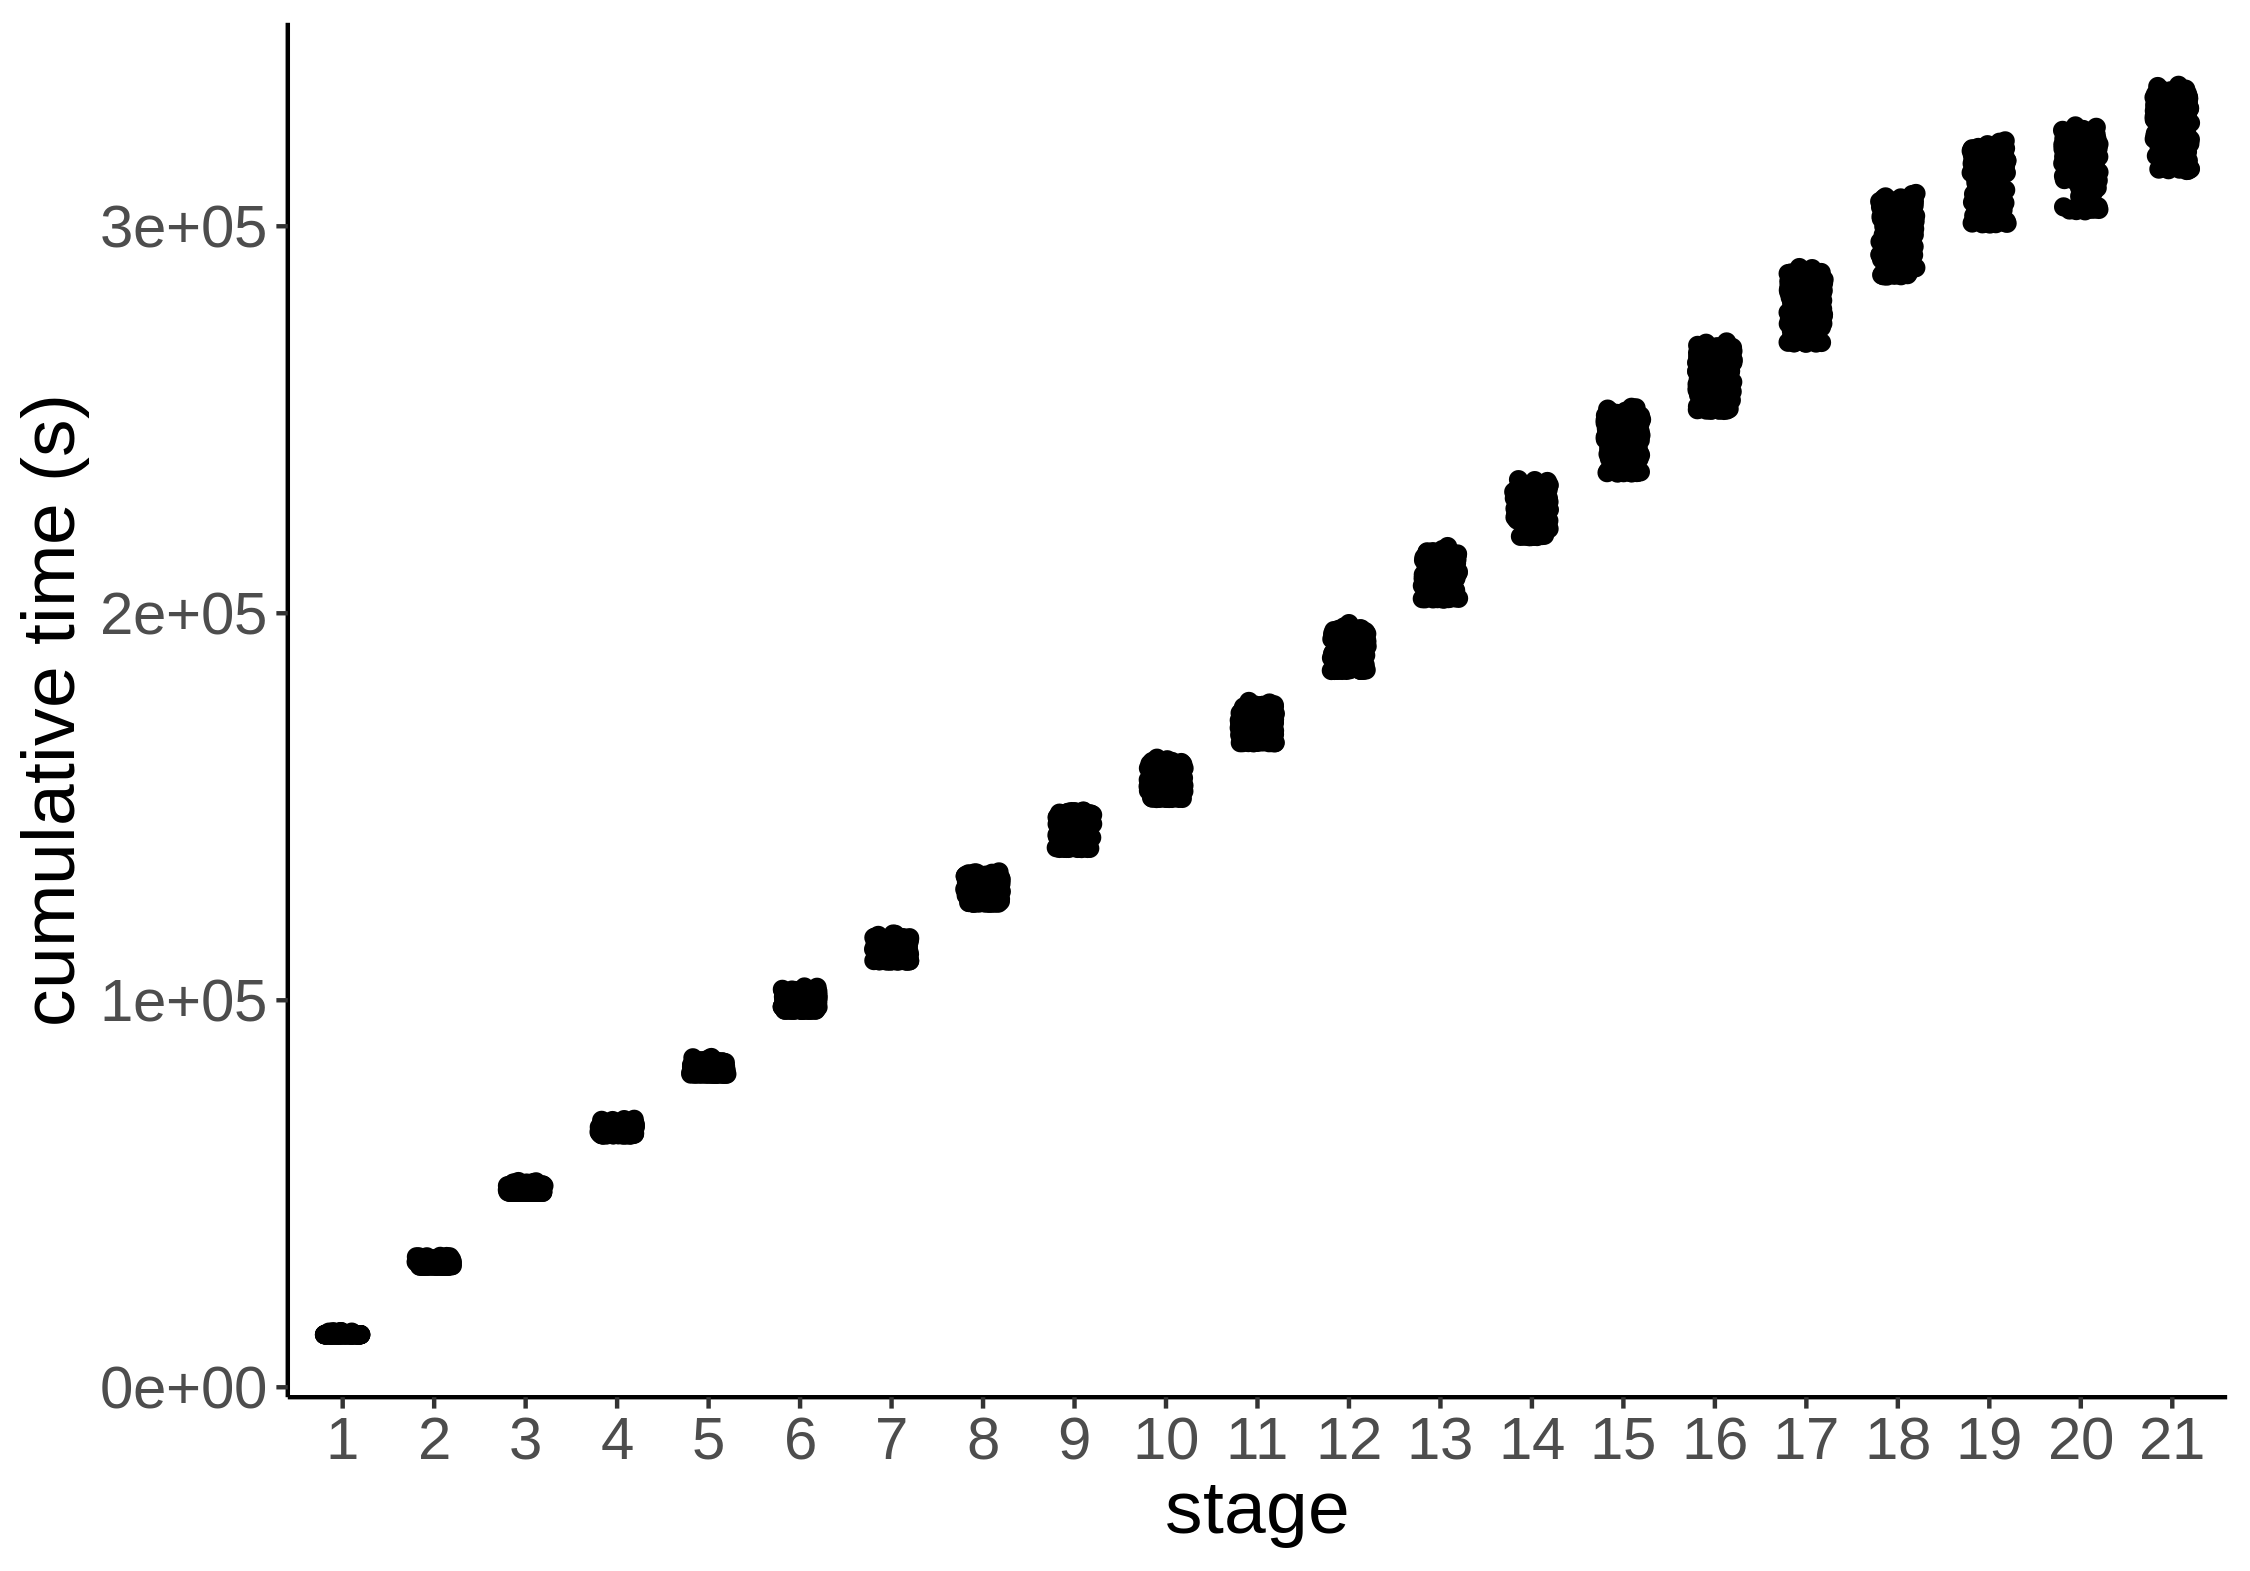
\includegraphics[scale=0.6]{fig/cumtime_stage.png}
  \caption{Scatterplot of cumulative time by stage. Each point corresponds to a rider's cumulative time at the corresponding stage.}
  \label{fig:cumtime}
\end{figure}


One alternative to cumulative time is the time difference of every rider to the race leader at every stage. A visual inspection of Figure \ref{fig:timediff_stage}, which shows how time differences vary through stage, suggests a linear relationship between stage and time difference. As was the case of cumulative time, the variance of the time difference also increases with stage---for similar reasons. Although time difference also resulst in a combinatorially complicated structure, it is not nearly as complicated as the one induced by the cumulative time. The model proposed in Section \ref{sec:stats} addresses these issues. \\



\begin{figure}[h]
  \centering
  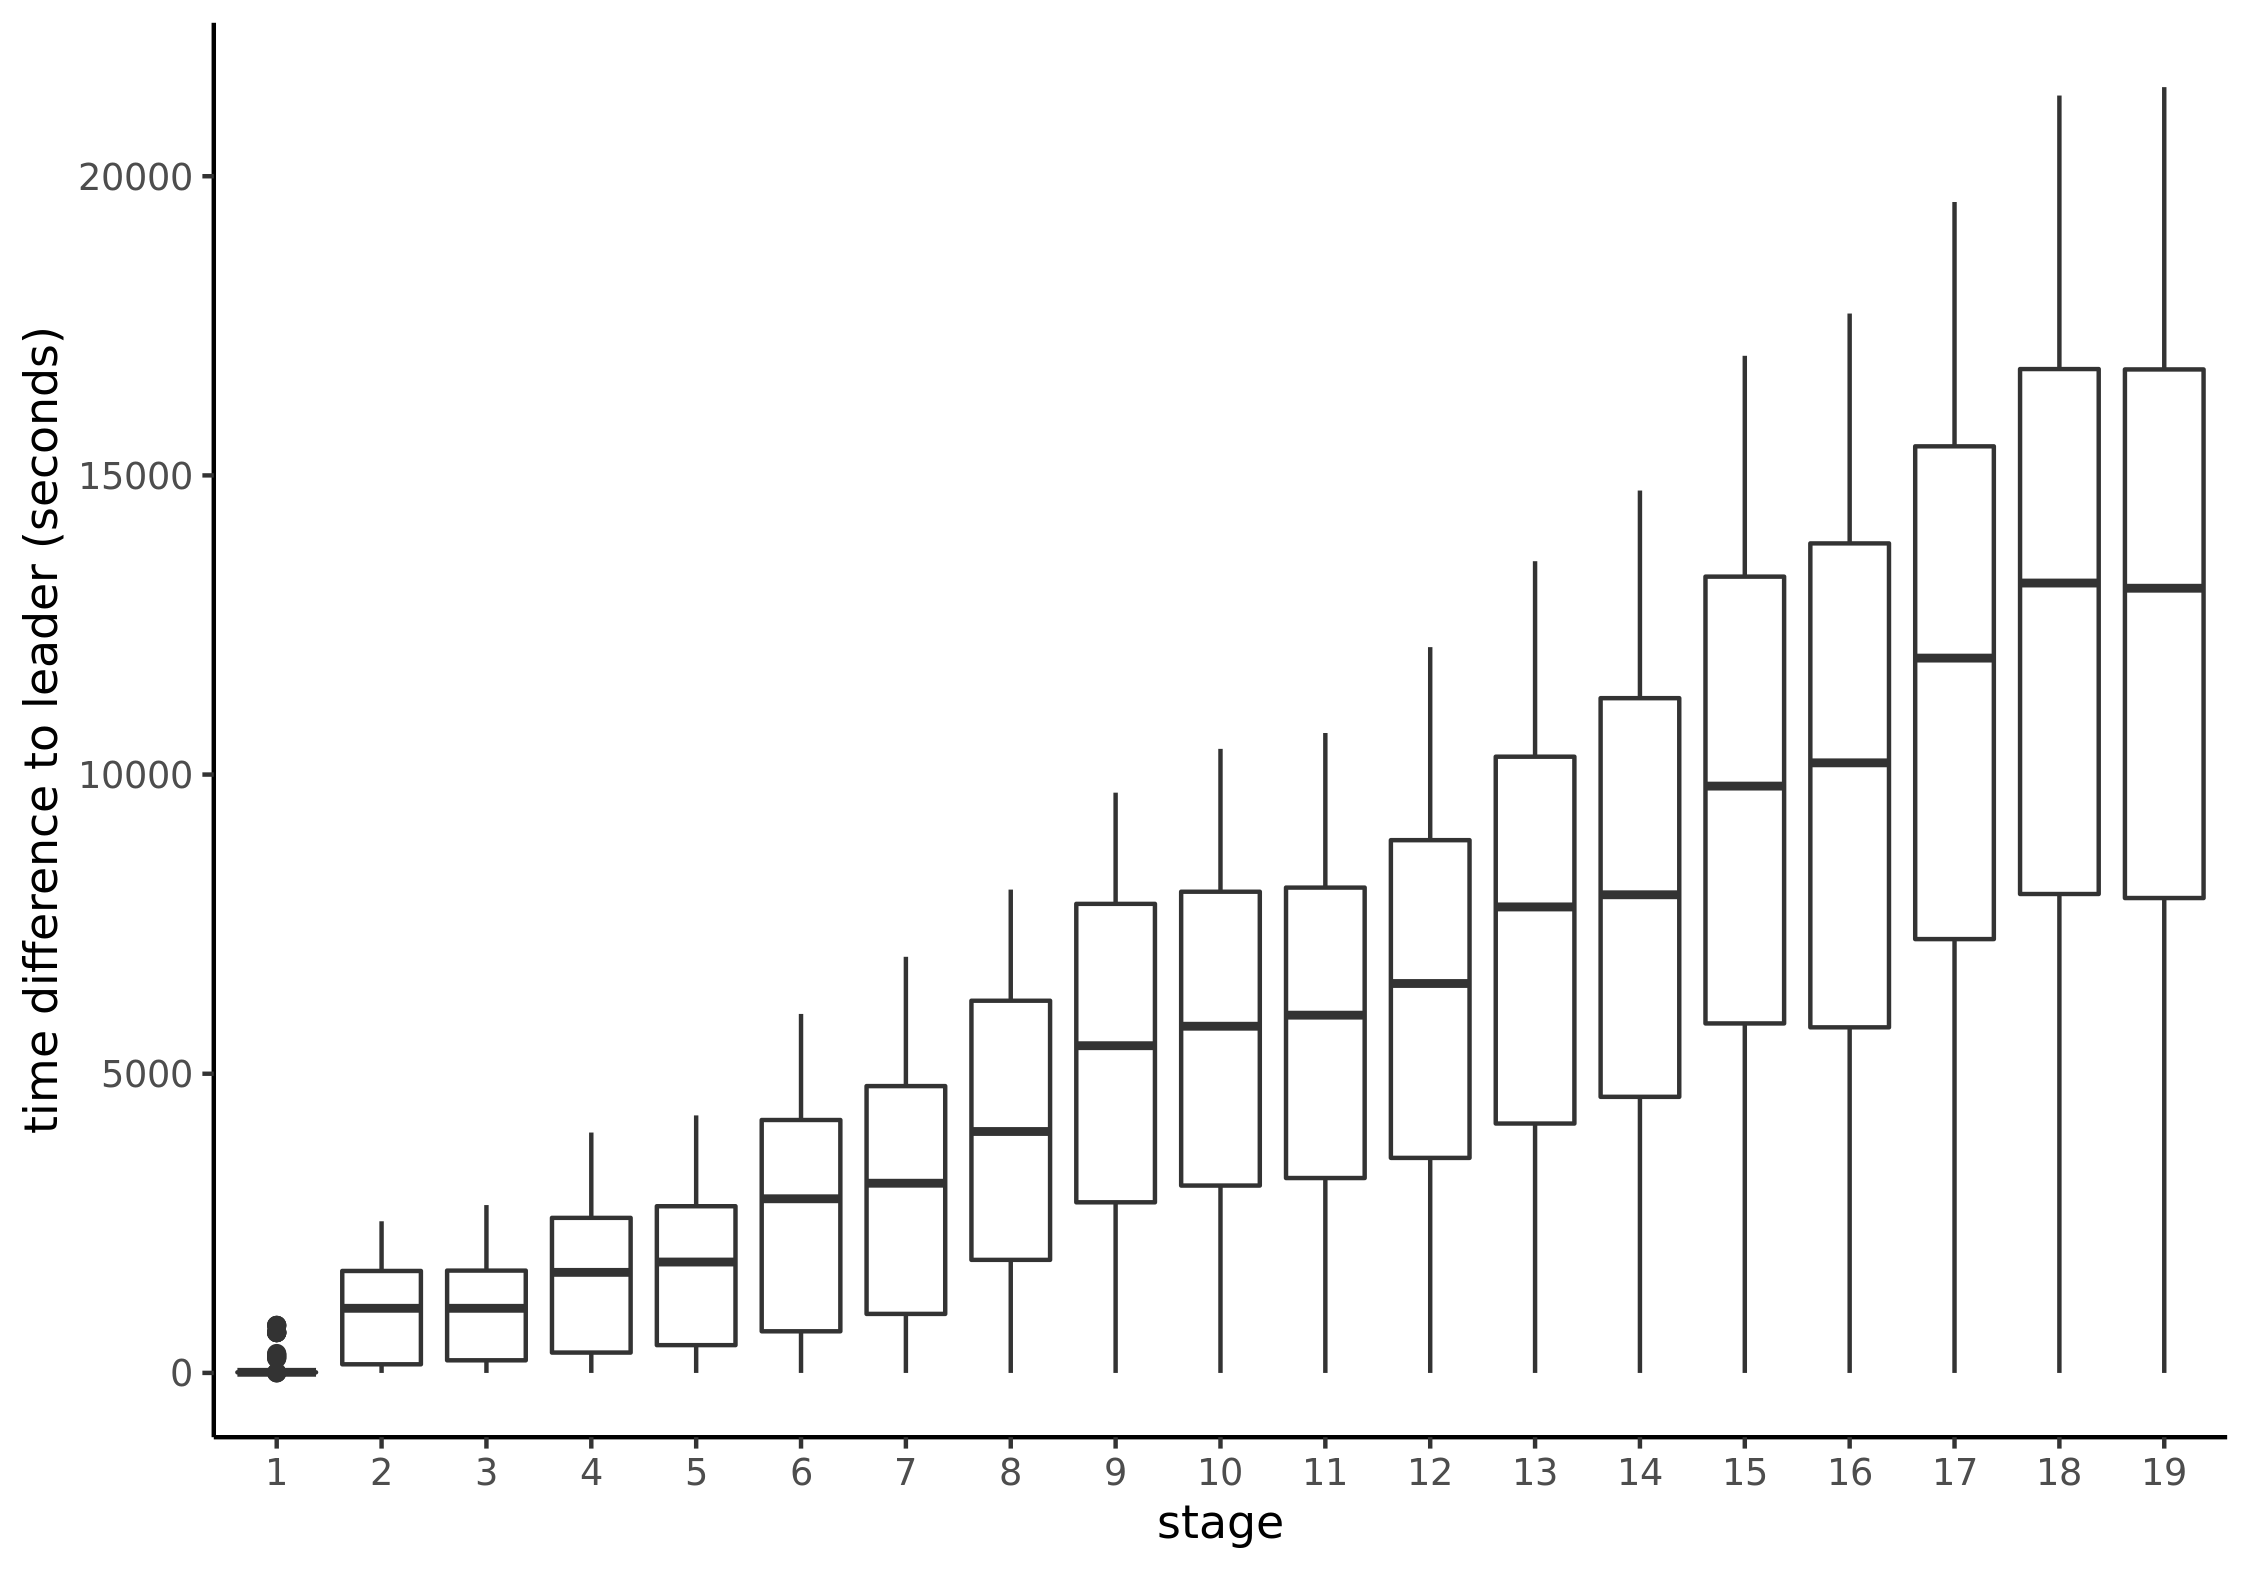
\includegraphics[scale=0.6]{fig/timediff_stage.png}
  \caption{Boxplots of time difference to leader for every stage. The variability in the time difference increases as stages progress.}
  \label{fig:timediff_stage}
\end{figure}



%\begin{figure}[h]
%  \centering
%  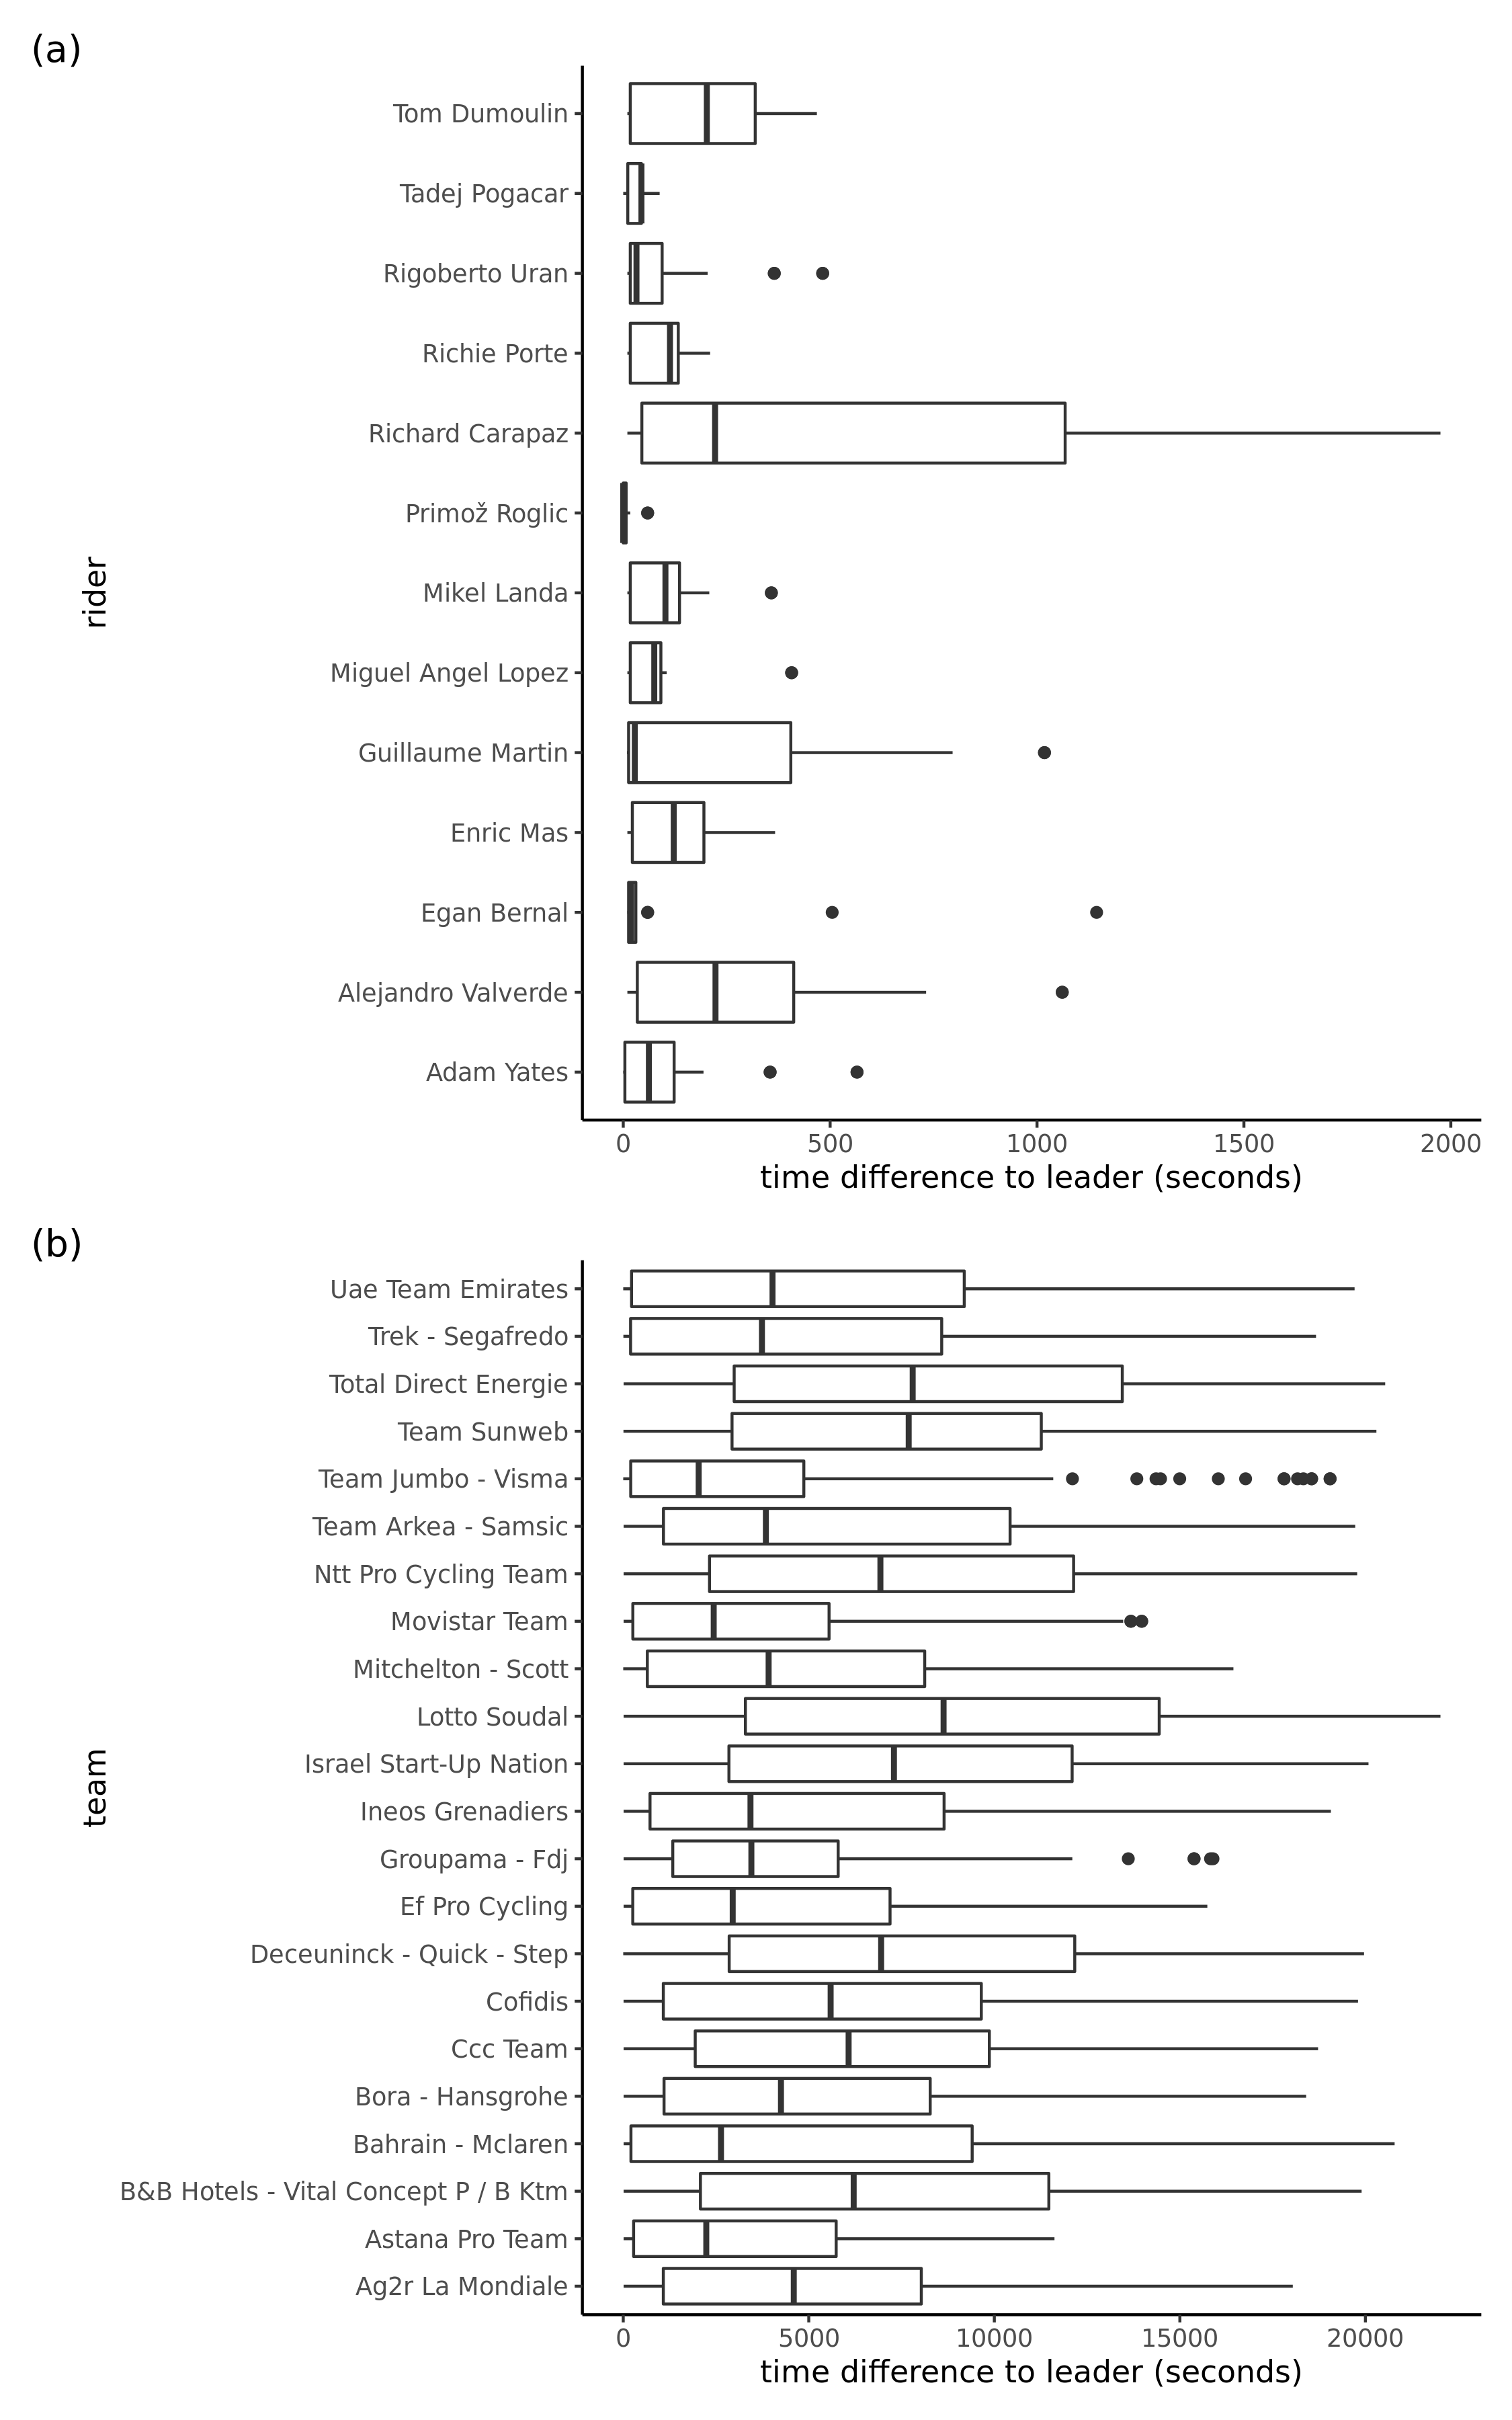
\includegraphics[scale=0.4]{fig/timediff_contender_team.png}
%  \caption{Boxplots of time difference to leader for every top contender and team. Contenders seem to vary more between them than teams.}
%  \label{fig:timediff_contender_team}
%\end{figure}

Figures \ref{fig:timediff_contender} and \ref{fig:timediff_team} suggest that time differences vary between the top contenders\footnote{These were determined by looking up the team leaders and favorites prior to the race.} of the Tour, and slightly between the teams as well. The model proposed in Section \ref{sec:stats} takes these two variables into account.


\begin{figure}[h]
  \centering
  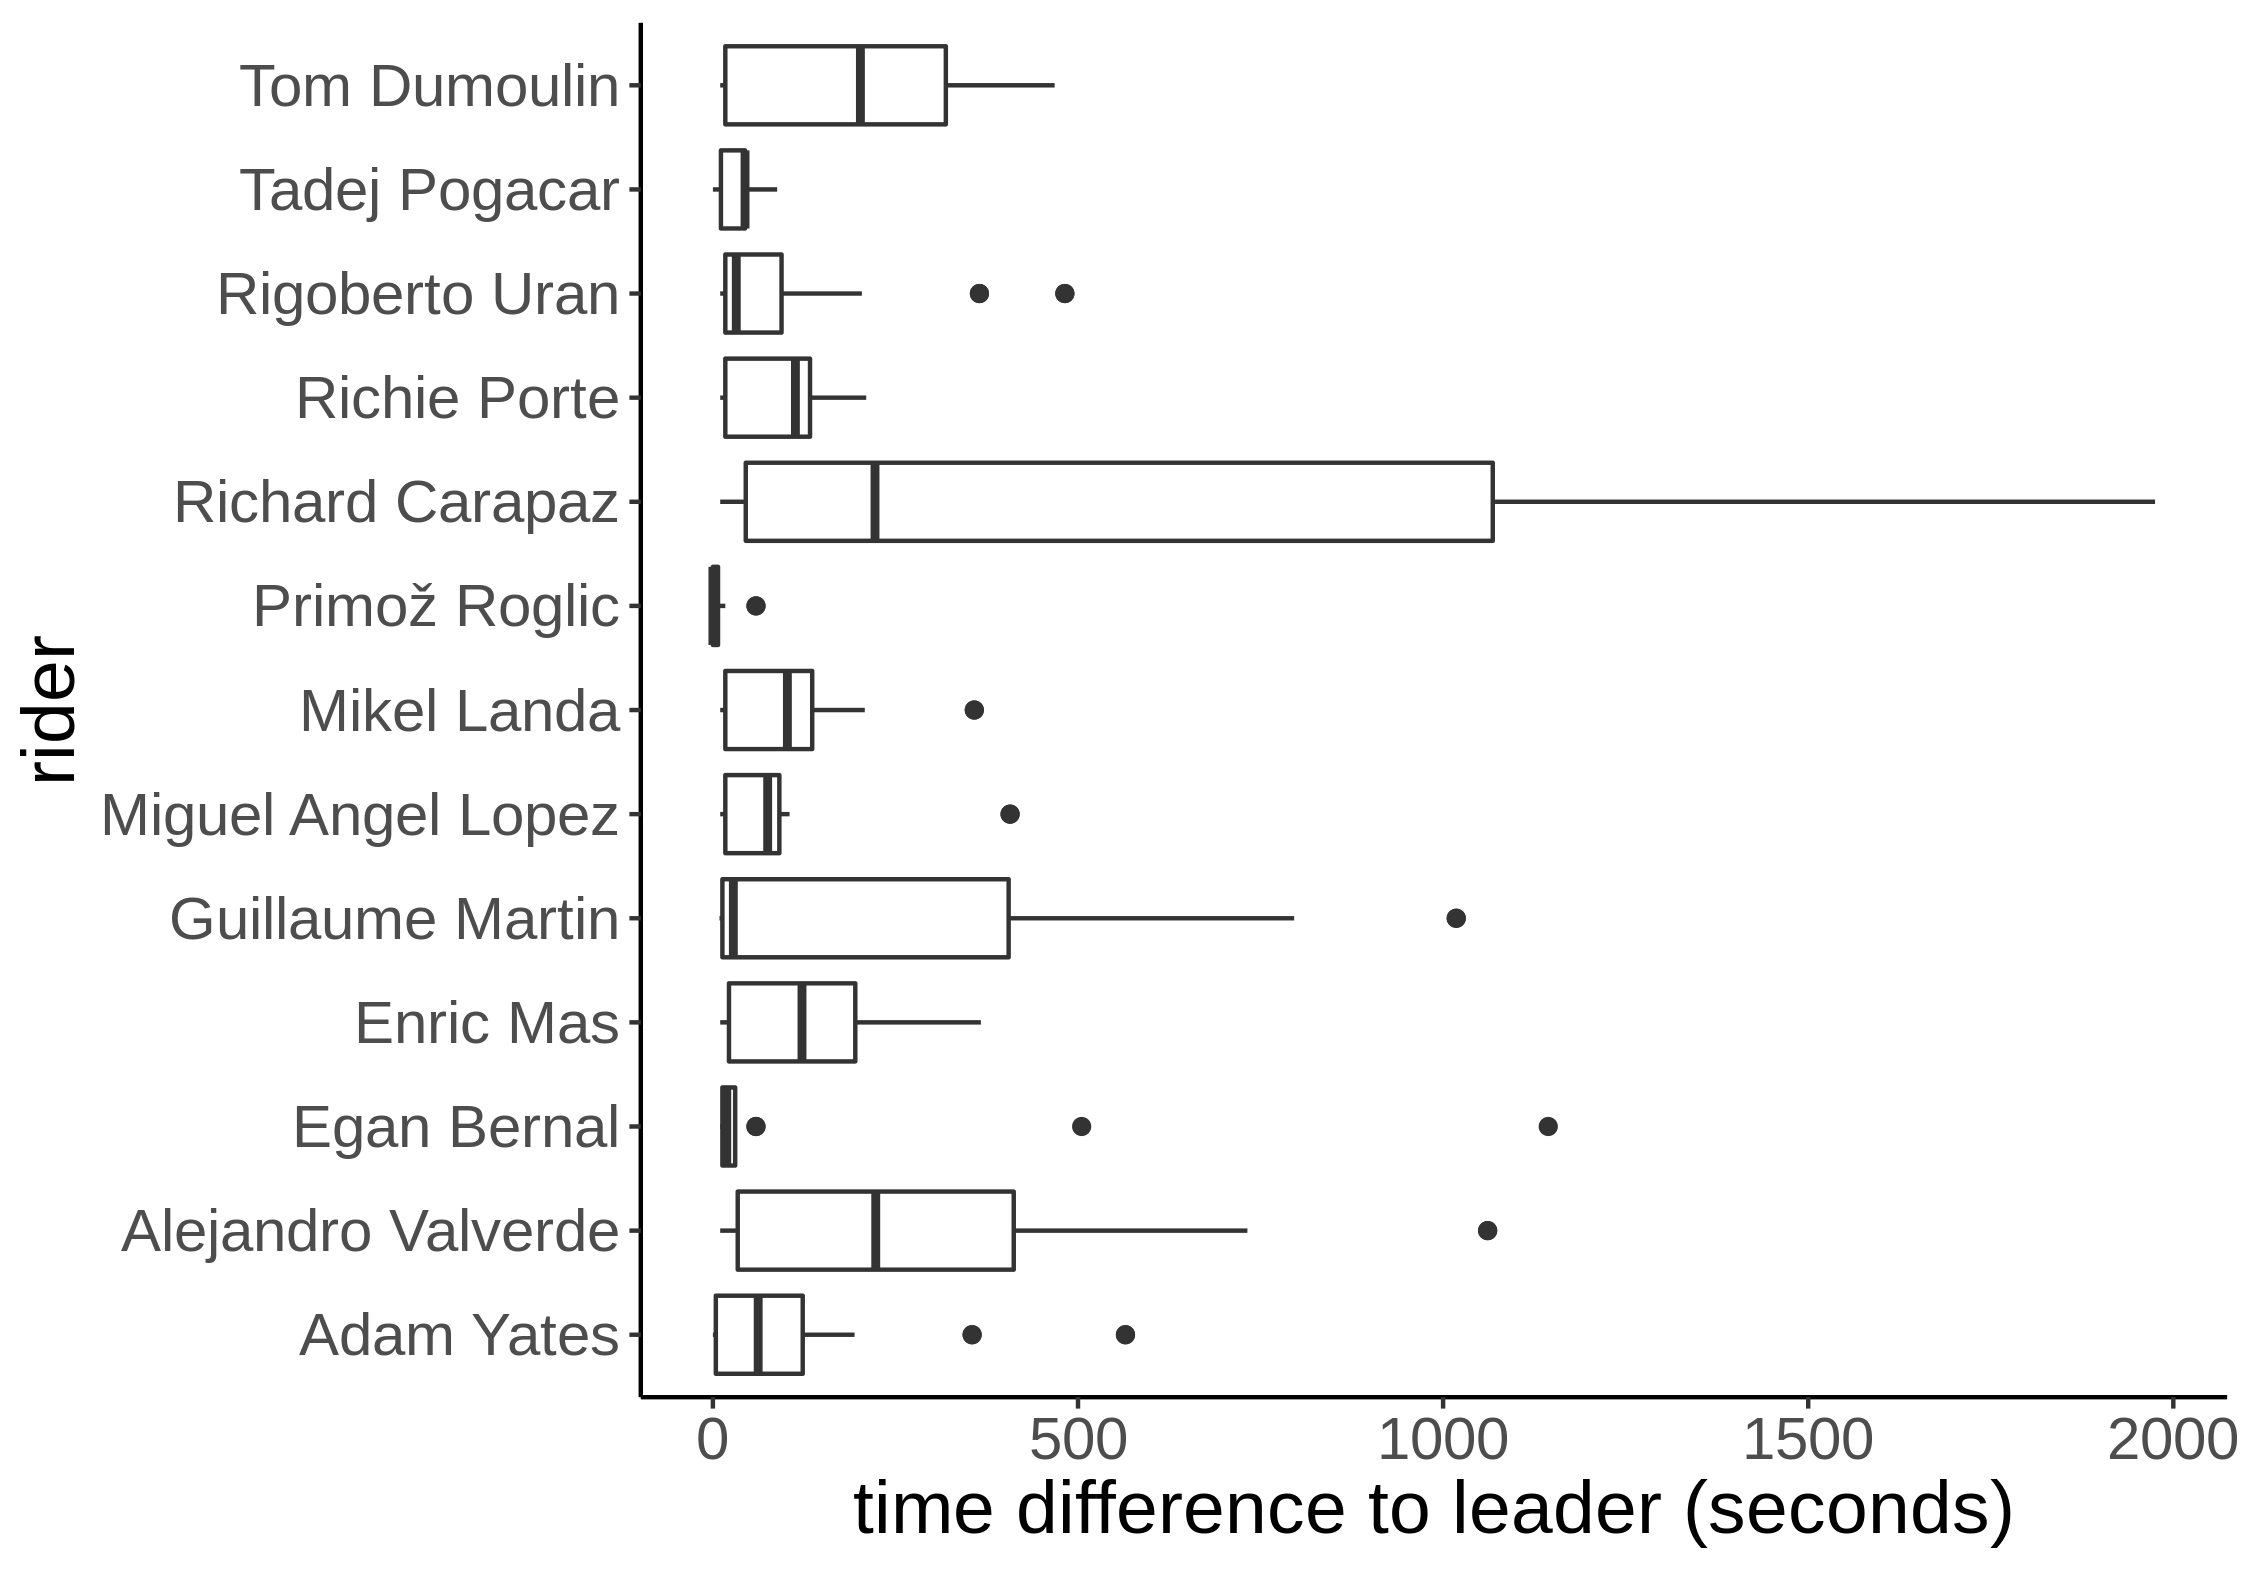
\includegraphics[scale=0.5]{fig/timediff_contender.png}
  \caption{Boxplots of time difference to leader for every top contender. Contenders seem to vary between them.}
  \label{fig:timediff_contender}
\end{figure}


\begin{figure}[h]
  \centering
  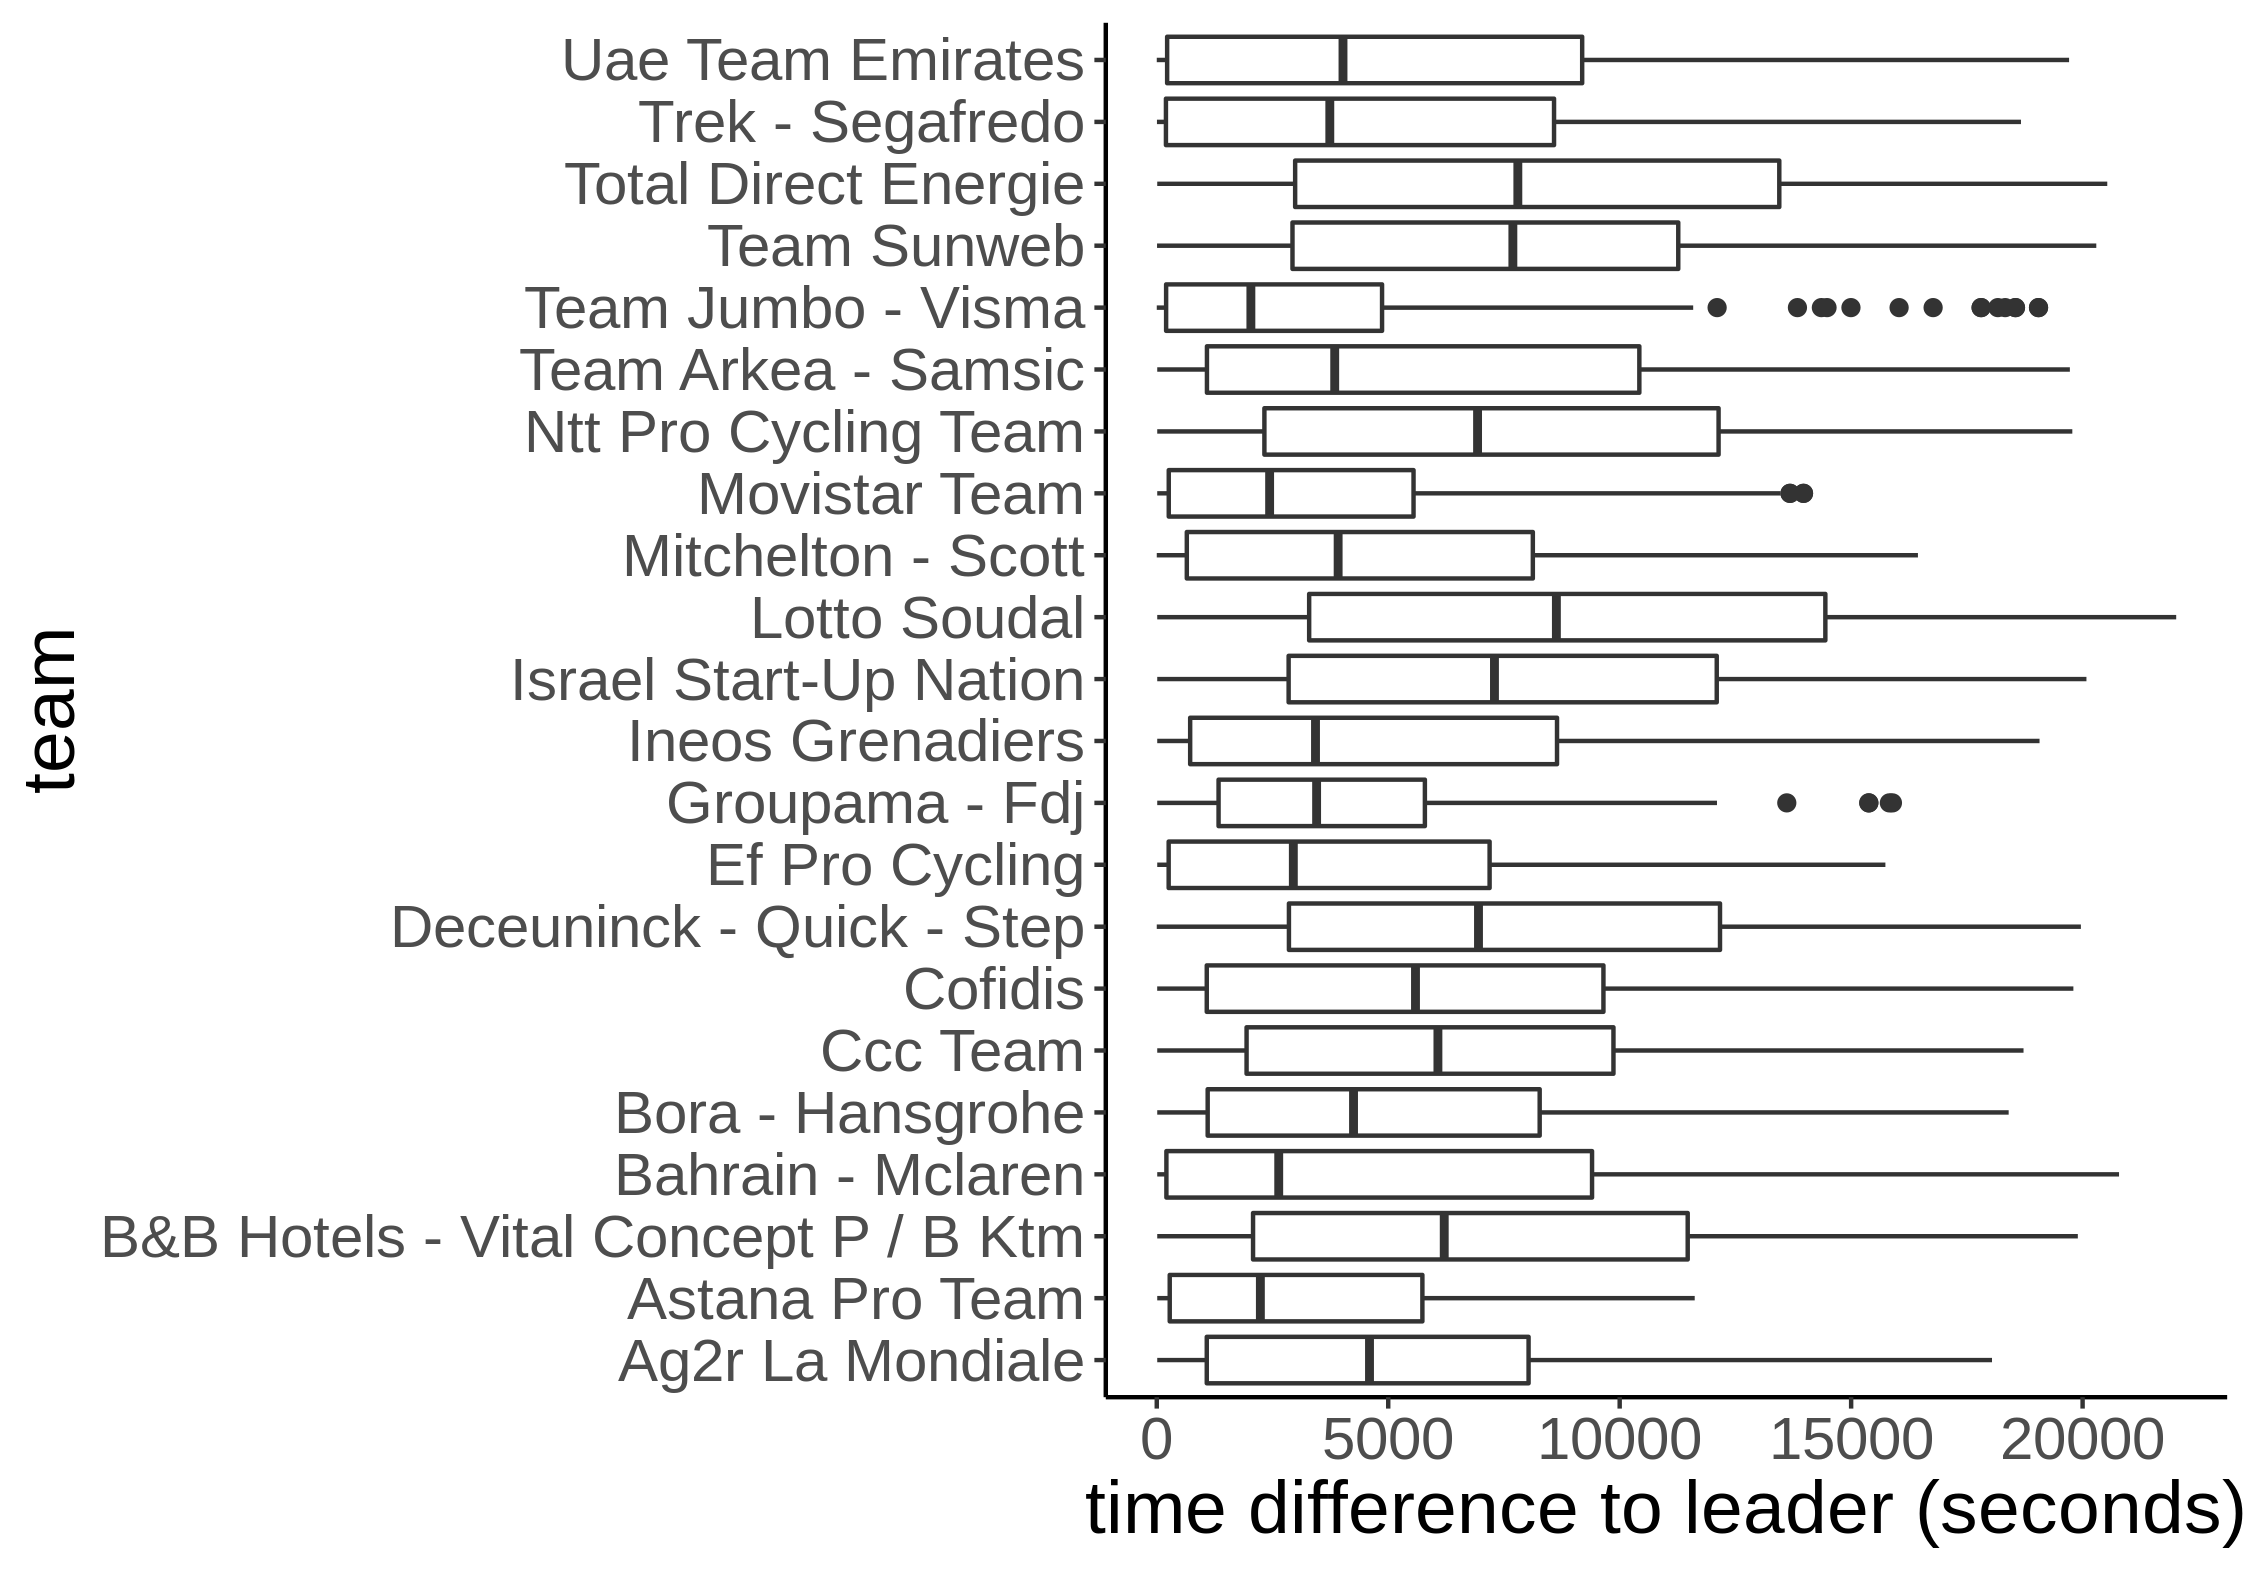
\includegraphics[scale=0.5]{fig/timediff_team.png}
  \caption{Boxplots of time difference to leader for every team. Contenders seem to vary more between them than teams.}
  \label{fig:timediff_team}
\end{figure}



\FloatBarrier


\section{Statistical methodologies} \label{sec:stats}

In this section, a zero-inflated probability model is proposed to study the time differences of riders. The model is then modified to account for combinatorial restrictions. Two response functions are proposed to fit the model to the data.



\subsection{Tweedie distribution}

There are two issues when dealing with the time differences. First, there is a non-zero probability of the time difference being zero. Indeed, at each stage there will be at least one observation equal to zero---namely, the leader of the race. Second, there \textit{has} to be at least one observation equal to zero at each stage. \\


To deal with the first issue, we propose modeling the time differences with a \textit{compound Poisson-Gamma} model \citep{tweedie1984, jorgensen1987}, which is defined as follows. Let $N \sim \distPoiss(\lambda)$ and define
\[
  Y \given N = \begin{cases}
    0, & N = 0, \\
    \gamma_{N, b}, & N > 0,
  \end{cases}
\]
where $\gamma_{N, b} \sim \distGamma(N, b)$. The marginal distribution of $Y$ is a compound Poisson-Gamma distribution with parameters $\lambda$ and $b$, denoted $Y \sim \distNamed{CPG}(\lambda, b)$. Observe that $Y$ has a non-zero probability of being zero. Specifically,
\[
  P(Y = 0) = P(N = 0) = \exp \{ -\lambda \}.
\]
When $N > 0$, $\gamma_{N, b}$ can be thought of as adding $N$ \iid $\distExp(b)$ distributions. More generally, one can add $N$ \iid $\distGamma(a, b)$ distributions \citep[see][]{withers2011}. For the purposes of this report, however, we assume the simpler case of adding exponential distributions. This has the benefit of having one less parameter to fit without losing much flexibility. In that case, it is easy to prove that
\[
  \EE [Y] = \frac{\lambda}{b}.
\]
The marginal density of $Y$ can be calculated in closed form.

\bnprop
  Let $Y \sim \distNamed{CPG}(\lambda, b)$. Then
  \[
    p(y; \lambda, b) = \exp\{ -\lambda \} \delta(y) + b \lambda \exp \{ -\lambda - by \} \sum_{n=0}^\infty \frac{(b y \lambda)^n}{(n+1)! n!}. \label{eq:cpg-pdf}
  \]
  where $\delta(y)$ is the Dirac $\delta$-function.
\enprop
The proof follows from the law of total probability. \cite[See][for example]{ozturk1981}. The sum in Eqn. \refeq{eq:cpg-pdf} converges quickly due to the denominator growing much faster than the numerator \citep{withers2011}. \\


What makes the compound Poisson-Gamma attractive from a regression perspective is that it is an \textit{exponential dispersion model}. A random variable $Y$ is said to be an exponential dispersion model if its density can be expressed as
\[
  p(y; \theta, \sigma^2) = \kappa(\sigma^2, y) \exp \left\{ \frac{\theta y - A(\theta)}{\sigma^2} \right\}.
\]
The mean of an exponential dispersion model is $\mu = A'(\theta)$, and we denote $Y \sim \distNamed{ED}(\mu, \sigma^2)$. Furthermore, if $Y \sim \distNamed{ED}(\mu, \sigma^2)$ then $\var (Y) = \sigma^2 V(\mu)$, where $V(\mu) = A''((A')^{-1}(\mu))$ is the variance function of $Y$. A special case of exponential dispersion models is the \textit{Tweedie family of distributions}. A random variable is said to follow a Tweedie distribution with power parameter $p$ if $Y \sim \distNamed{ED}(\mu, \sigma^2)$ and $V(\mu) = \mu^p$ for some $p \in \reals$, in which case we denote $Y \sim \distNamed{Tweedie}(\mu, \sigma^2, p)$. Compound Gamma-Poisson models are actually Tweedie distributions. \\

\bnprop
  If $Y \sim \distNamed{CPG}(\lambda, b)$ then $Y \sim \distNamed{Tweedie}(\mu, \sigma^2, p = 1.5)$ with
  \[
    \mu &= \frac{\lambda}{b}, \\
    \sigma^2 &= \frac{2}{\sqrt{\lambda b}}.
  \]
\enprop

A proof can be found in \citep{jorgensen1994} by substituting $\alpha = -1$ in their analysis. \cite{smyth1996} shows that, for the case of a $\distNamed{Tweedie}(\mu, \sigma^2, p = 1.5)$ distribution,
\[
  \theta = -2 \mu^{-\half}, \quad A(\theta) = - 4 \theta^{-1}. \label{eq:canonical}
\]
In summary, by modeling the time difference of riders to the race leader with a compound Poisson-Gamma model, we actually end up with a Tweedie distribution.



\subsection{Random component}

Maximum-likelihood estimates (MLE) for the parameters of a Tweedie distribution can be approximated realiably \citep{ozturk1981, withers2011}. This, combined with its close relationship to exponential families, means that it is amenable to be used in generalized linear models. \\

In our case, let $Y_n^k$ denote the time difference of rider $n$ to the race leader at stage $k$, $n=1, ..., N, \, k = 1, ...K$. We will assume that $Y_n^k \distiid \distNamed{Tweedie}(\mu_n^k, \sigma^2, p = 1.5)$. For presentation purposes, we assume there are the same number of riders by stage to avoid using $N_k$. This has no impact on the analysis. \\

We also assume independence both between riders and within stages for a given rider. Between riders, each rider is assumed to try to race in as little time as possible regardless of other riders. Within riders, it would be intuitive to assume that a given rider's time difference in a stage has a lot of influence on the next stage. This is not necessarily so, however: it is not uncommon for riders to launch attacks and reduce their time difference considerably, or alternatively to break down in a climb and lose plenty of time.\footnote{This happended to the defending champion, Egan Bernal, while ascending the Grand Colombier in stage 15. He lost 7 minutes on his 59 seconds gap and subsequently abandoned the race.} Finally, it is also possible for two riders to have the same time difference, and even for two riders to have a time difference of zero. Specifically, final sprints at some stages can result in riders having the same time. Although it is unlikely that two riders will be tied as leaders, it is not technically impossible.\footnote{In 1989, Greg LeMond won the Tour with a time difference of a mere 8 seconds.} \\

The likelihood of the data under this setting can be written down as
\[
  p(y_1^1, ..., y_N^K; \, \mu, \sigma^2) = \prod_{k=1}^K \prod_{n=1}^N p(y_n^k; \, \mu_n^k, \sigma^2),
\]
where $\mu = (\mu_1^1, ..., \mu_N^K)^\top$ and $p(y_n^k; \, \mu_n^k, \sigma^2)$ is the Tweedie likelihood. However, as we mentioned before, there is an additional combinatorial restriction: at each stage, there has to be at least one rider with a time difference of zero. We overcome this by adding a multiplicative factor to the likelihood that ensures this restriction is satisfied:
\[
  p(y_1^1, ..., y_N^K; \, \mu, \sigma^2) = \prod_{k=1}^K \left[ \prod_{n=1}^N p(y_n^k; \, \mu_n^k, \sigma^2) \right] \ind_{\{ 0\}} (y_{(N)}^k),
\]
where $\ind_A(x) = 1$ if $x \in A$ and 0 otherwise and $y_{(N)}^k = \min \{y_1^k, ..., y_N^k \}$. The additional factor is 1 when each stage has an observation that is zero and 0 otherwise. The log-likelihood is more illuminating:
\[
  \log p(y_1^1, ..., y_N^K; \, \mu, \sigma^2) = \sum_{k=1}^K \sum_{n=1}^N \log p(y_n^k; \, \mu_n^k, \sigma^2) + \sum_{k=1}^K \log \ind_{\{ 0\}} (y_{(N)}^k). \label{eq:loglike}
\]
The first term in Eqn. \refeq{eq:loglike} is the log-likelihood of \iid Tweedie observations. The second term can be thought of as a penalty: it takes the value of 0 when each stage has an observation that is zero, and the value of $-\infty$ otherwise. In the case a stage does not have an observation that is zero, the MLE is not defined. \\


Note that our data satisfy the combinatorial constraint by construction. Indeed, that is the reason we considered it in the first place. Hence, the log-likelihood of the model parameters---which will be introduced briefly---given our data is not going to have the additional penaly term, which is going to equal zero. This means that we can do regular MLE without worrying about the combinatorial constraint. \\


Finally, it should be noted that the variance of $Y \sim \distNamed{Tweedie}(\mu, \sigma^2, p = 1.5)$ can be written as
\[
  \var (Y) = \sigma^2 \mu^{1.5}.
\]
In our setting, this will also account for the non-constant variance.


\subsection{Systematic component}


Based on the exploratory data analysis of Section \ref{sec:eda}, we will use stage, distance, team, and rider as predictors. The last two variables are categorical, and so it is necessary to create indicator variables for each category (minus one reference category). Because there are around 150 riders and 22 teams, this would entail having $150+22 = 172$ covariates. Even though the training data consist of over 3,000 observations, we consider the risk of overfitting to be too large. On the other hand, however, it is necessary to produce predictions at the rider level to be able to answer the main research question. \\

To remedy this, we instead include indicator variables only for the 13 top contenders of the Tour, and aggregate the other riders into an ``Other'' category. Not only does this strike a balance between having predictions at the rider level and not overfitting, but it is also justified in the context of the Tour: not all riders in the Tour are actively trying to win the general classification. Some are aiming to win some of the other races in the Tour (points and mountains), while some are there only to support the team leader. \\

The linear predictor will thus be
\[
  \eta_n^k = \beta_0 + \beta^\top x_n^k, \quad \beta = (\beta_1, ..., \beta_{36})^\top,
\]
where $\beta_1$ corresponds to the stage number; $\beta_2$ corresponds to the stage distance; $\beta_3$ through $\beta_{23}$ correspond to the indicator variables of the different teams; and $\beta_{24}$ through $\beta_{36}$ correspond to the indicator variables of the different contenders, or favorite riders.




\subsection{Response function}



Motivated by Figure \ref{fig:timediff_stage}, we would like to equate the linear predictor with the mean of the response variable $\mu_n^k$ to leverage the linear relationship between the stage number and the time differences. However, $\mu_n^k$ has to be non-negative, and the linear predictor need not be positive. Indeed, its sign depends on the values of $\beta$. Hence, using an identity response function is not immediatly possible. We leave exploring ways to enforce a linear relationship between stage number and time differences for future work. \\

One alternative is to use a log response function,
\[
  \log \mu_n^k = \eta_n^k, \quad n = 1, ..., N, \, k = 1, ..., K. \label{eq:log-response}
\]
Under the log response function, the covariates have a multiplicative effect on the mean of the response, which makes the model easier to interpret. Another alternative is to use the (scaled) canonical response which, following Eqn. \refeq{eq:canonical}, for this case is given by
\[
  (\mu_n^k)^{-\half} = \eta_n^k, \quad n = 1, ..., N, \, k = 1, ..., K. \label{eq:canonical-response}
\]
Under the canonical response, the log-likelihood is concave and thus iterative optimization methods have convergence guarantees.



\section{Results} \label{sec:results}


We fit two models to the data. Both model the time difference as a Tweedie distribution, but differ in the response function used. Specifically, one model uses the log response function (\refeq{eq:log-response}) and the other model uses the canonical response function (\refeq{eq:canonical-response}). The code to generate all figures and fit the models can be found at \url{https://github.com/GiankDiluvi/tdf-2020}. \\


Figure \ref{fig:fitted_predicted} shows a comparison of the true time differences against the fitted and predicted values of both models. Regardless of the response function, the compound Gamma-Poisson models capture the increase in variability as a function of stage. However, variability is underestimated at earlier stages and overestimated at later stages, most likely as a result of not using the identity link. Both models tend to estimate the time difference as either too large or too small. This is probably due to the contender dummy variables: the model can make more accurate predictions for the contenders, who will usually have smaller time differences. The other riders are differentiated only by team, and so their predictions are much larger and closer between each other. One potential way to remedy this would be to further split the ``Others'' group into two or more categories reflecting the performance of the riders (e.g. high, medium, and low performers). In any case, predicted values seem to be well within the expected range. \\



\begin{figure}[h]
  \centering
  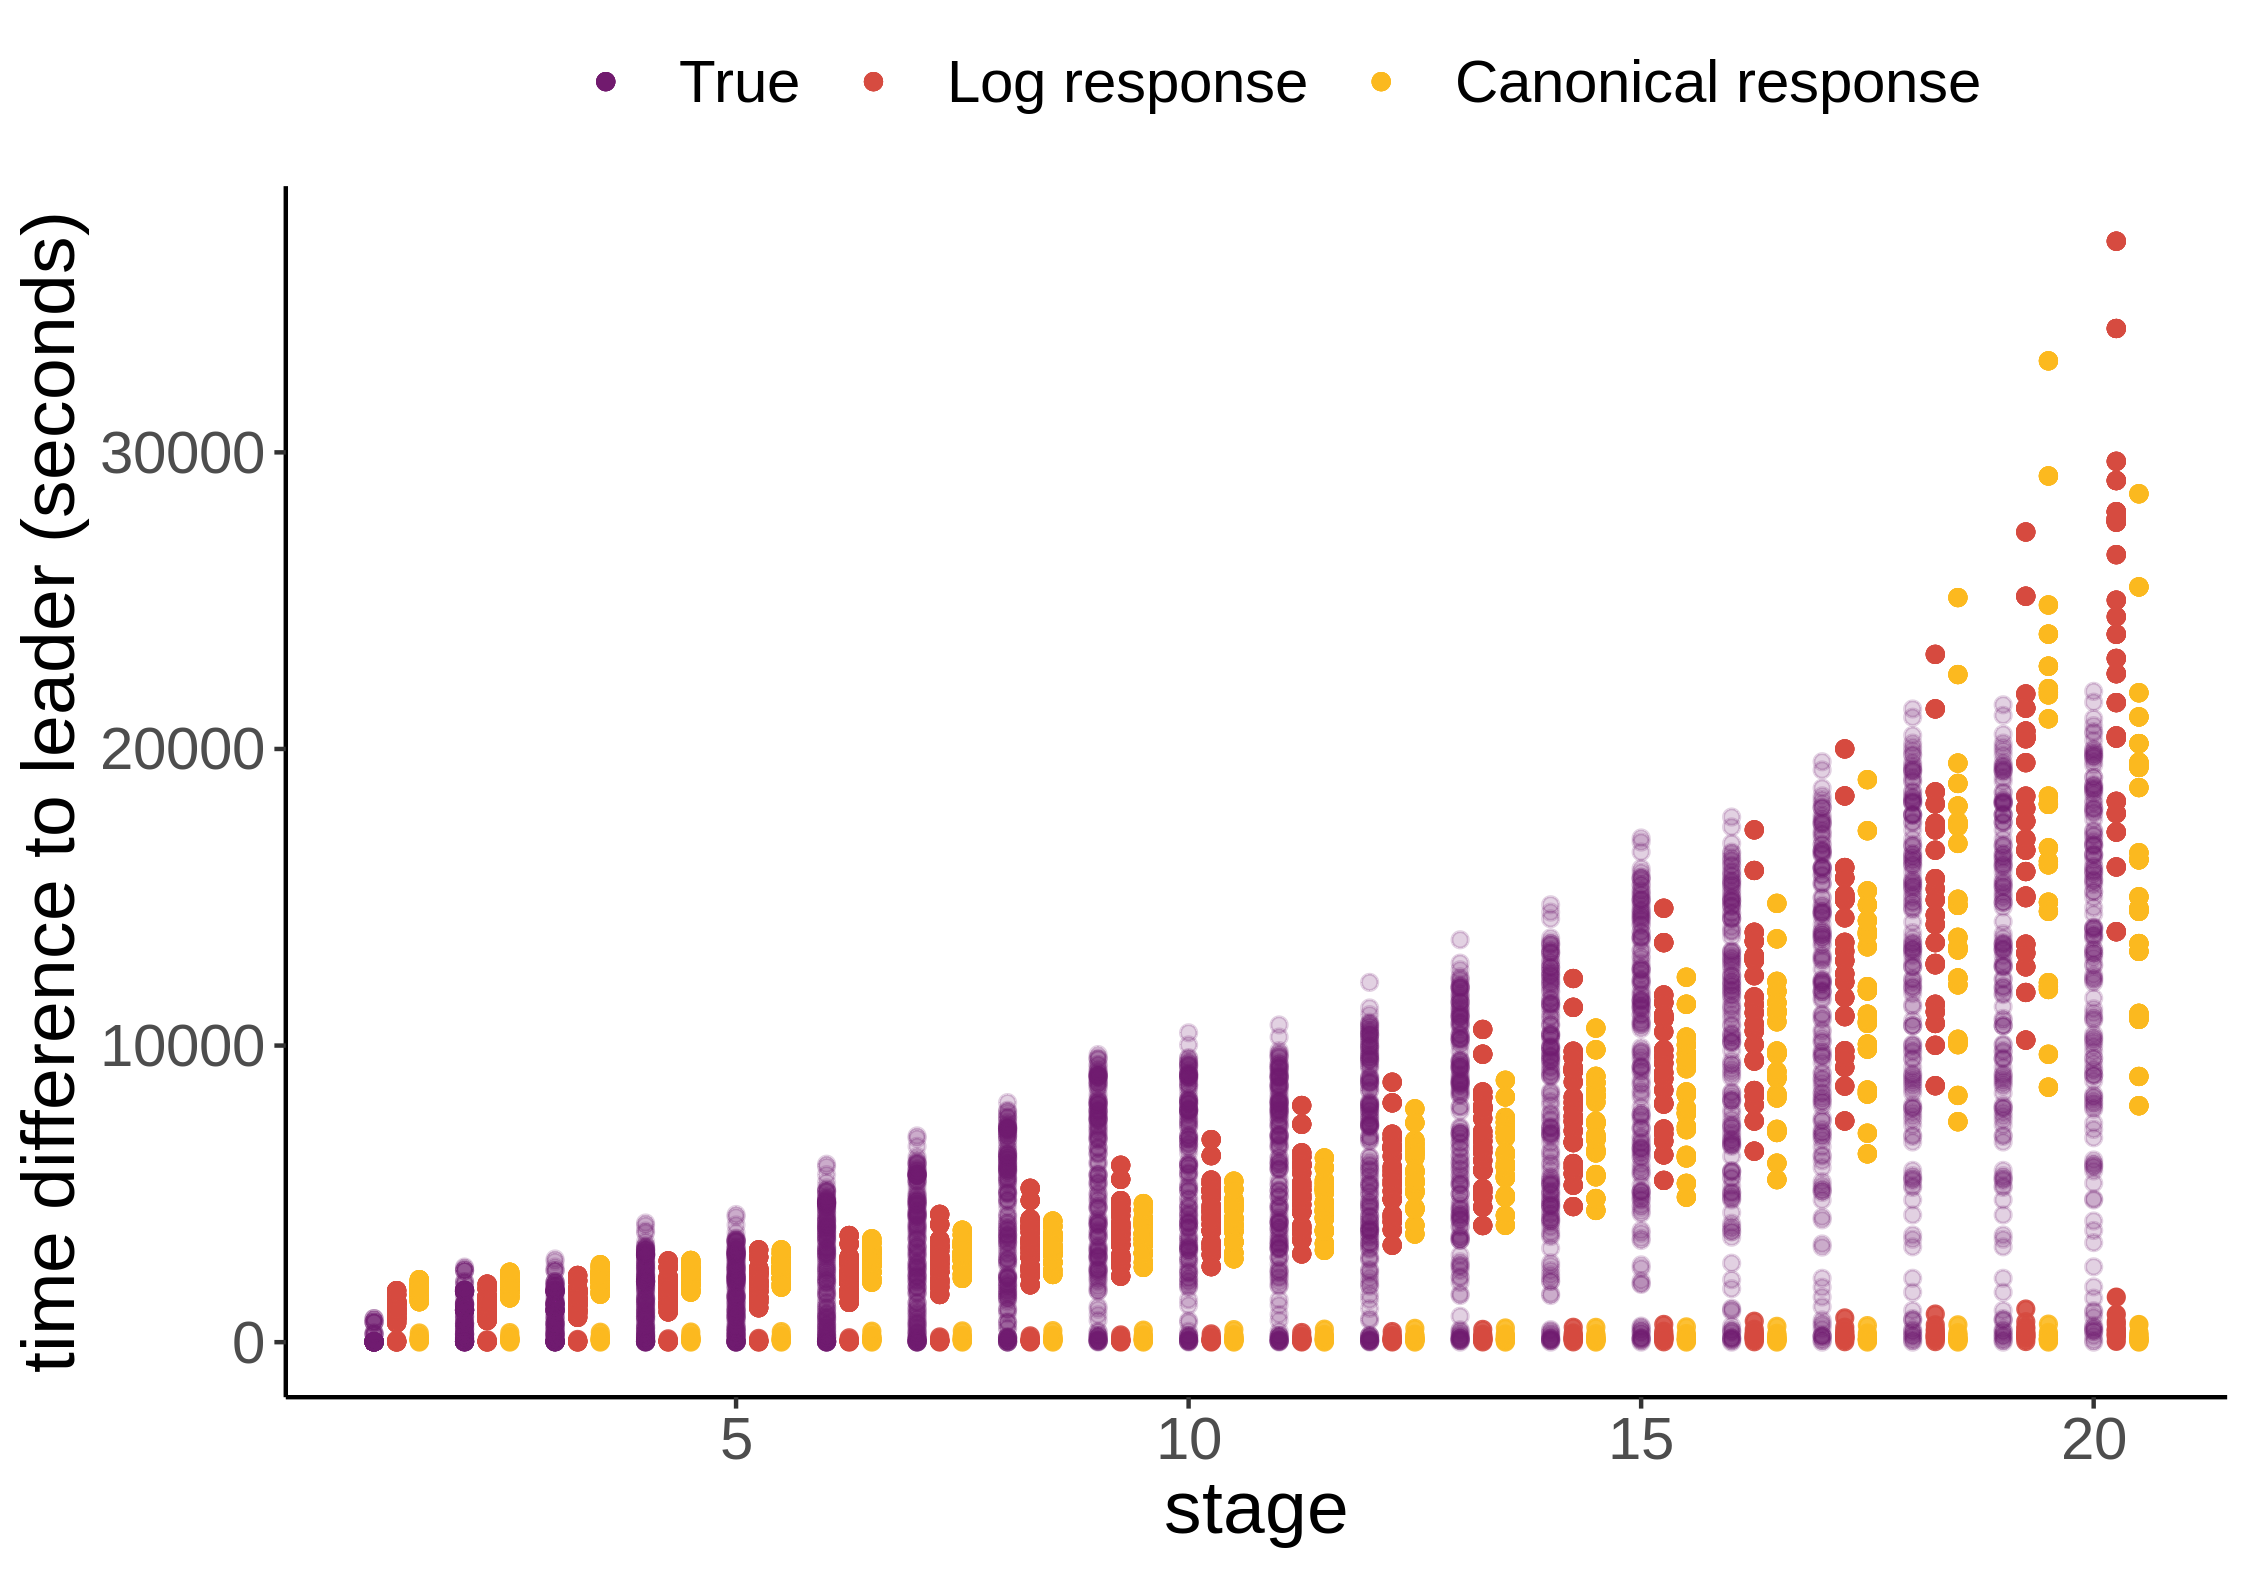
\includegraphics[scale=0.65]{fig/fitted_predicted_comparison.png}
  \caption{Comparison of fitted (stages 1 to 19) and predicted (stage 20) values of both models, with color by response function, against the true values. The compound Poisson-Gamma model successfully captures the increasing variability of observations.}
  \label{fig:fitted_predicted}
\end{figure}



To answer the research question, Table \ref{table:results} shows both model's predictions for the top 10 riders. Neither model was able to predict Tadej Pogačar as the Tour's winner, although both placed him in second place. However, both  models assigned Pogačar a large probability of winning (i.e. of his time difference being zero, which can be calculated from the estimated parameters). Regarding the probabilities of winning, the model with the canonical response tends to assign larger probabilities in general, which means that the underlying Tweedie distribution has more mass concentrated on zero. With the exception of 10th place, both models seem to have recovered the top contenders, albeit not in exact order. \\


%\begin{table}[ht]
%\centering
%\begin{tabular}{lccc}
%\textbf{Rider}     & \textbf{True ranking} & \textbf{Predicted ranking} & \textbf{\begin{tabular}[c]{@{}c@{}}Predicted probability\\  of winning\end{tabular}} \\ \hline
%Tadej Pogačar      & 1                     & 2                          & 0.228                                     \\
%Primož Roglič      & 2                     & 1                          & 0.552                                     \\
%Richie Porte       & 3                     & 7                          & 0.111                                     \\
%Mikel Landa        & 4                     & 6                          & 0.112                                     \\
%Enric Mas          & 5                     & 8                          & 0.095                                     \\
%Miguel Ángel López & 6                     & 3                          & 0.182                                     \\
%Tom Dumoulin       & 7                     & 10                         & 0.052                                     \\
%Rigoberto Urán     & 8                     & 4                          & 0.159                                     \\
%Adam Yates         & 9                     & 5                          & 0.152                                     \\
%Damiano Caruso     & 10                    & 67                         & $<$0.0001                         \\ \hline
%\end{tabular}
%\caption{Top 10 riders of the 2020 Tour de France. For each rider, its ranking and predicted ranking are shown, along with the predicted probability of winning.}
%\label{table:results}
%\end{table}




\begin{table}[ht]
\centering
\begin{tabular}{lc|cc|cc}
\multirow{2}{*}{\textbf{Rider}} & \multirow{2}{*}{\textbf{\begin{tabular}[c]{@{}c@{}}True \\ ranking\end{tabular}}} & \multicolumn{2}{c|}{\textbf{Log response function}}                                           & \multicolumn{2}{c}{\textbf{Canonical response function}}                                      \\ \cline{3-6}
                                &                                                                                   & \textbf{Ranking} & \textbf{\begin{tabular}[c]{@{}c@{}}Probability\\  of winning\end{tabular}} & \textbf{Ranking} & \textbf{\begin{tabular}[c]{@{}c@{}}Probability\\  of winning\end{tabular}} \\ \hline
Tadej Pogačar                   & 1                                                                                 & 2                & 0.228                                                                      & 2                & 0.545                                                                      \\
Primož Roglič                   & 2                                                                                 & 1                & 0.552                                                                      & 1                & 0.841                                                                      \\
Richie Porte                    & 3                                                                                 & 7                & 0.111                                                                      & 6                & 0.373                                                                      \\
Mikel Landa                     & 4                                                                                 & 6                & 0.112                                                                      & 7                & 0.373                                                                      \\
Enric Mas                       & 5                                                                                 & 8                & 0.095                                                                      & 8                & 0.334                                                                      \\
Miguel A. López                 & 6                                                                                 & 3                & 0.182                                                                      & 3                & 0.475                                                                      \\
Tom Dumoulin                    & 7                                                                                 & 10               & 0.052                                                                      & 9                & 0.241                                                                      \\
Rigoberto Uran                  & 8                                                                                 & 4                & 0.159                                                                      & 4                & 0.409                                                                      \\
Adam Yates                      & 9                                                                                 & 5                & 0.152                                                                      & 5                & 0.394                                                                      \\
Damiano Caruso                  & 10                                                                                & 67               & \textless{}0.0001                                                          & 67               & \textless{}0.0001                                                          \\ \hline
\end{tabular}
\caption{Top 10 riders of the 2020 Tour de France. For each rider, its true ranking and predicted ranking are shown, along with the predicted probability of winning for both models. The model that uses the canonical response function tends to assign larger probabilities to the time difference being zero.}
\label{table:results}
\end{table}




Figure \ref{fig:norm_res} shows the normalized residuals for both models. The vast majority of normalized residuals lie within 3 units from the origin. However, some normalized residuals for small fitted values are below the -3 bound for both models. The figure also suggests that the models overestimate when fitted values are large and underestimate when they are small, which is in line with Figure \ref{fig:fitted_predicted}. Again, this is likely due to the response functions not being the identity. The coefficients of the  model, along with the corresponding P-values, are shown in the Appendix. \\




\begin{figure}[h]
  \centering
  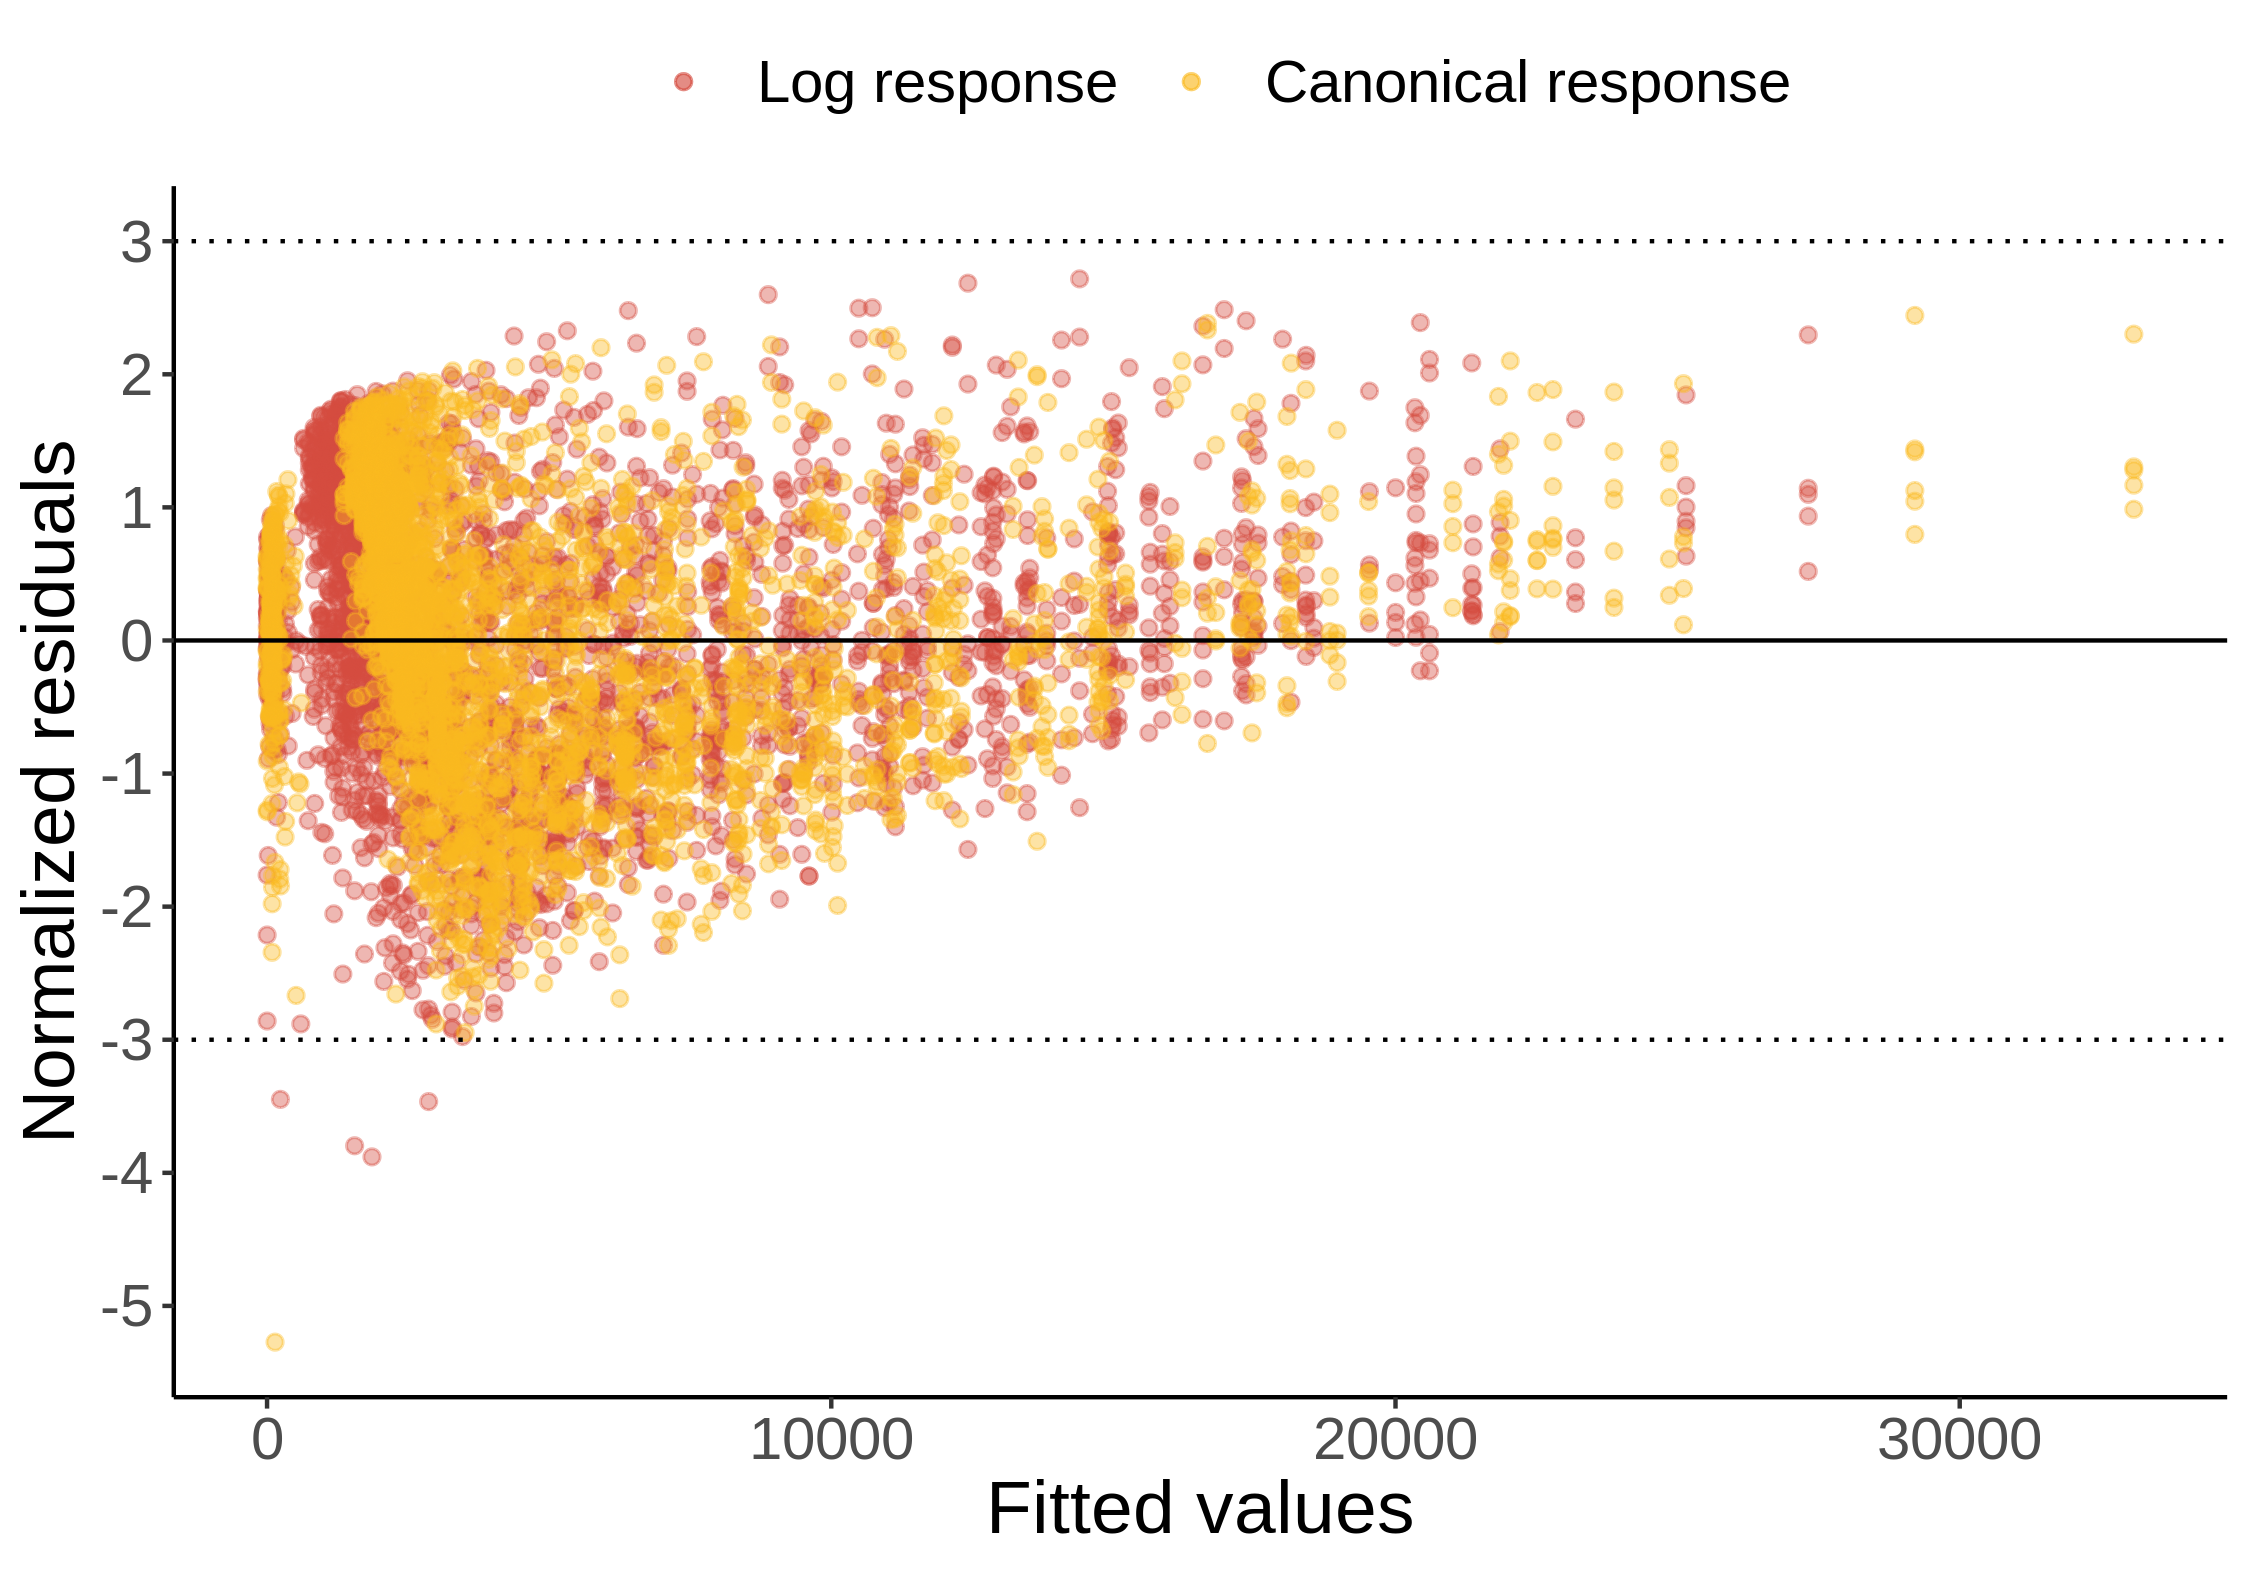
\includegraphics[scale=0.65]{fig/norm_res_comparison.png}
  \caption{Normalized residuals of the compound Poisson-Gamma models, with color by response function. The vast majority of values are well within the $\pm$ 3 bound. The models tend to overestimate when fitted values are small and underestimate when they are large.}
  \label{fig:norm_res}
\end{figure}


Both models generally agree on their results. Even though neither managed to predict Pogačar's victory, they both assigned non-trivial probabilities to his victory.


\section{Conclusion} \label{sec:conclusion}


We proposed a zero-inflated generalized linear model based on compound Gamma-Poisson and Tweedie distributions to model the time difference of each rider of the 2020 Tour de France to the Tour's leader at each stage. We suggested two possible response functions---logarithm and canonical---to associate the linear predictor---which included the stage number, distance, rider's team, and favorite riders---with the mean of the time difference, which led to two models. After fitting these two models, we found that both predicted favorite Primož Roglič to be the winner of the Tour. However, they both also assigned relatively large probabilities of winning to Tadej Pogačar, the actual winner of the Tour. In that sense, Pogačar's victory should not have been as much a surprise as it was. \\


One limitation of the model is that it cannot capture the linear relationship between the time difference and the stage number because the identity link would result in values of the linear predictor that are not attainable for the response mean. The impact of this limitation was discussed in previous sections, and boils down to an underestimation of the variability in the response for early stages, and an overestimation for later ones. One possible way to overcome this would be to restrict the values of the parameter associated with stage number to be non-negative, which would allow that covariate to linearly influence the response. Given the observed positive association between stage number and time difference, this might be reasonable. The rest of the parameters can be scaled using another response function, which would result in a non-linear model, or similarly restricted. Whether optimization methods are guaranteed to converge in this setting is also left for future work. Another alternative would be to use a Bayesian approach and directly incorporate the parameter restrictions into their prior distributions. Unfortunately, popular probabilistic programming languages such as \textsf{Stan} do not have a built-in Tweedie regression family, which would require the user to develop code to approximate the density. \\


Another limitation is that the model assumes independence between different stages of the same rider. This can be partly justified by the fact that riders can almost arbitrarily lose or win time difference at any given stage. However, it would be interesting to properly account for this longitudinal structure. Whether the gains in accuracy, if any, offset the increase in complexity is also left for future work. \\

Finally, a variable that was not included in the model and that might have had a significant impact is the type of stage. Some riders specialize in certain types of stages (such as mountain stages), and this can have a significant effect on their performance. However, the 20th stage in this year's Tour de France was the only time trial\footnote{Where riders race individually against the clock, usually in shorter routes that allow them to output more power throughout the stage.} of the whole Tour. Hence, there were no data on which to train the model for this stage type. Future work can explore including results from other Tours in the training data set, although how to account for missing and new riders is not clear. (Specifically, this year's Tour was Pogačar's first.) \\



\FloatBarrier
\clearpage
\small
\bibliographystyle{imsart-nameyear}
\bibliography{ref/tdf-2020.bib}

\clearpage
\appendix

\section{Coefficients and P-values}


Figures \ref{fig:log_coefficients} and \ref{fig:canonical_coefficients} show the coefficient estimates and P-values for both models. In both models stage and distance are significant at the 0.05 level, some teams are also significant, and most contenders are not. Both models were fit using \textsf{R} 4.0.3 \citep{R} in an ASUS ROG GL552VX computer with 64-bit Linux Mint 19.3, 8 GB of RAM memory, and an Intel Core i7-6700HQ CPU at 2.60GHz.

\begin{figure}[h]
  \centering
  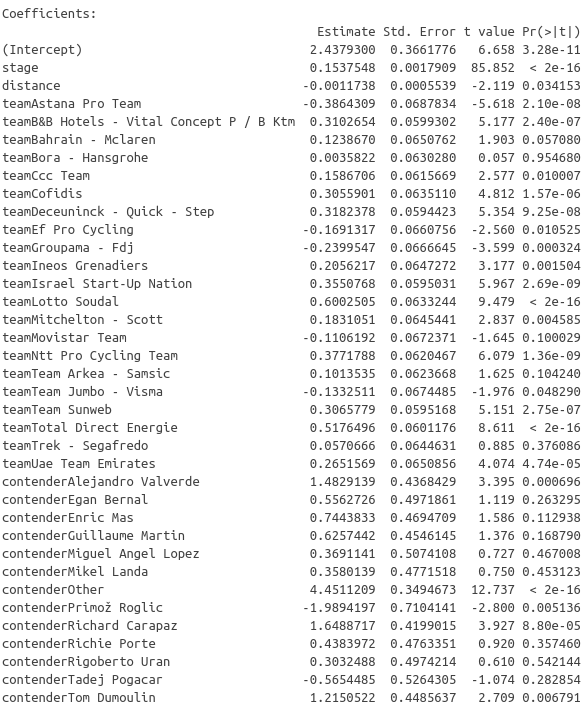
\includegraphics[scale=0.5]{fig/log_coefficients.png}
  \caption{Coefficient estimates, standard error, $t$-statistics, and P-values for the model with the log response function.}
  \label{fig:log_coefficients}
\end{figure}

\newpage


\begin{figure}[h]
  \centering
  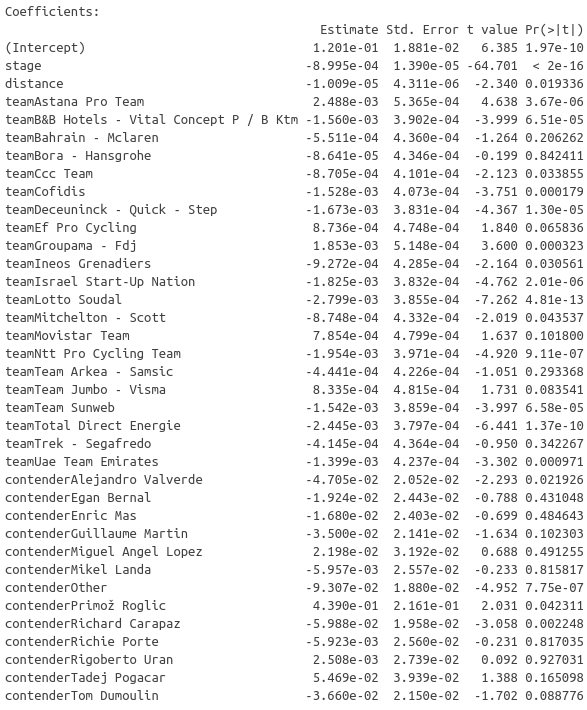
\includegraphics[scale=0.5]{fig/canonical_coefficients.png}
  \caption{Coefficient estimates, standard error, $t$-statistics, and P-values for the model with the canonical response function.}
  \label{fig:canonical_coefficients}
\end{figure}




\end{document}
